% 编译顺序: xelatex -> bibtex -> xelatex -> xelatex
% 国家自然科学基金NSFC面上项目申请书正文模板(2023年版)version1.0
% 声明:
% 注意!!!非国家自然科学基金委官方模版!!!由个人根据官方MsWord模版制作。本模版的作者尽力使本模版和官方模版生成的PDF文件视觉效果大致一样,然而,并不保证本模版有用,也不对使用本模版造成的任何直接或间接后果负责。 不得将本模版用于商用或获取经济利益。本模版可以自由修改以满足用户自己的需要。但是如果要传播本模版,则只能传播未经修改的版本。使用本模版意味着同意上述声明。
% 强烈建议自己对照官方MsWord模板确认格式和文字是否一致,尤其是蓝字部分。
% 如有问题,可以发邮件询问原作者 ryanzz@foxmail.com,或本版本的修改者 yimian.dai@gmail.com


\documentclass[12pt,UTF8,AutoFakeBold=3,a4paper]{ctexart} %默认小四号字。允许楷体粗体。
\usepackage{nsfc}


%%%%%%%%%%%%%%%%%%%%%%%%%%% 自定义命令 %%%%%%%%%%%%%%%%%%%%%%%%%%%%%

\newcommand{\expect}{\mathbb{E}}
\newcommand{\code}[1]{\ensuremath{\mathsf{#1}}}
% \newcommand{\ccode}[1]{{\ttfamily {#1}}}
\newcommand{\ccode}[1]{ \lstinline|#1| }
\newcommand{\mln}{\Phi}
\newcommand{\sentence}{\Gamma}
\newcommand{\defsentence}{\Upsilon}
\newcommand{\generalsentence}{{\widehat{\sentence}}}
\newcommand{\recursivesentence}{{\widetilde{\sentence}}}
\newcommand{\fotwoformula}{\psi}
\newcommand{\formula}{\psi}
\newcommand{\mlnformula}{\alpha}
\newcommand{\formulas}{\Psi}
\newcommand{\weight}{w}
\newcommand{\vecweight}{\mathbf{\weight}}
\newcommand{\negweight}{\bar{w}}
\newcommand{\negvecweight}{\mathbf{\negweight}}
\newcommand{\World}{\Omega}
\newcommand{\world}{\omega}
\newcommand{\wfomc}{WFOMC}
\newcommand{\wfoms}{WFOMS}
\newcommand{\fastwfomc}{FastWFOMC}
\newcommand{\fomc}{FOMC}
\newcommand{\symwfomc}{\ensuremath{\mathsf{WFOMC}}}
\newcommand{\symfomc}{\ensuremath{\mathsf{FOMC}}}
\newcommand{\wmc}{WMC}
\newcommand{\wms}{WMS}
\newcommand{\csp}{\ensuremath{\mathsf{CSP}}}
\newcommand{\symwmc}{\ensuremath{\mathsf{WMC}}}
\newcommand{\symwms}{\ensuremath{\mathsf{WMS}}}
\newcommand{\symmc}{\ensuremath{\mathsf{MC}}}
\newcommand{\symms}{\ensuremath{\mathsf{MS}}}
\newcommand{\fo}{\mathbf{FO}}
\newcommand{\fotwo}{\ensuremath{\mathbf{FO}^2}}
\newcommand{\fothree}{\ensuremath{\mathbf{FO}^3}}
\newcommand{\ctwo}{\ensuremath{\mathbf{C}^2}}
\newcommand{\setcell}{\mathbf{C}}
\newcommand{\config}{\mathcal{C}}
\newcommand{\indicator}{\mathds{1}}
\newcommand{\indices}{\mathbf{N}}
\newcommand{\cardinality}{\mathbf{N}}
\newcommand{\domain}{\Delta}
\newcommand{\dftdomain}{\mathcal{D}}
\newcommand{\dftvec}{\mathbf{M}}
\newcommand{\vecn}{\mathbf{n}}
\newcommand{\vecm}{\mathbf{m}}
\newcommand{\veck}{\mathbf{k}}
\newcommand{\vecg}{\mathbf{g}}
\newcommand{\vecj}{\mathbf{j}}
\newcommand{\vecy}{\mathbf{y}}
\newcommand{\vecx}{\mathbf{x}}
\newcommand{\vech}{\mathbf{h}}
\newcommand{\vecu}{\mathbf{u}}
\newcommand{\innerprod}[2]{\langle#1,#2\rangle}
\newcommand{\nat}{\mathbb{N}}
\newcommand{\real}{\mathbb{R}}
\newcommand{\complex}{\mathbb{C}}
\newcommand{\dftmln}{\mln_{\textrm{DFT}}}
\newcommand{\generaor}{\mathcal{G}}
\newcommand{\pro}{\mathbb{P}}
\newcommand{\extformula}{\varphi}
\newcommand{\rejsentence}{\sentence_{\rm{reject}}}
\newcommand{\rejlineage}{\eta_{\rm{reject}}}
\newcommand{\pair}[1]{{(#1)}}
\newcommand{\tuple}[1]{(#1)}
\newcommand{\constraint}{\mathcal{C}}
\newcommand{\fomodels}[2]{\mathcal{M}_{#1, #2}}
\newcommand{\tree}{\ensuremath{\mathsf{T}}}
\newcommand{\dtree}{\ensuremath{\mathsf{DT}}}
\newcommand{\treesum}{\ensuremath{\mathsf{TS}}}
\newcommand{\ufotwo}{\ensuremath{\mathbf{UFO}^2}}
\newcommand{\distinctpair}{\Omega}
\newcommand{\onetypes}{\mathcal{U}}
\newcommand{\twotypes}{\mathcal{B}}
\newcommand{\structure}{\mathcal{A}}
\newcommand{\typeweight}[1]{\langle \weight, \negweight\rangle(#1)}
\newcommand{\generalonetype}{\widetilde{\tau}}
\newcommand{\sumweight}{\mathcal{W}}
\newcommand{\condvariables}[2]{\bar{#1}^{(#2)}}
\newcommand{\cofola}{\ensuremath{\mathsf{SCF}}}
\newcommand{\rmp}{RMP}
\newcommand{\symrmp}{\ensuremath{\mathsf{RMP}}}
\newcommand{\fastrmp}{\textbf{Fast-RMP}}
\newcommand{\approxwfomc}{\textbf{ApproxWFOMC}}
\newcommand{\symapproxwfomc}{\ensuremath{\mathsf{ApproxWFOMC}}}
\newcommand{\fastapproxwfomc}{\textbf{Fast-ApproxWFOMC}}
\newcommand{\symfastapproxwfomc}{\ensuremath{\mathsf{Fast-ApproxWFOMC}}}
\newcommand{\polytope}{\mathcal{P}}
\newcommand{\Vars}{\mathcal{V}}
\newcommand{\pred}{r}
\newcommand{\Preds}{\mathcal{R}}
\newcommand{\partitionfunc}{Z}
\newcommand{\sentences}{\Gamma}
\newcommand{\integer}{\mathbb{Z}}
\newcommand{\dftrmp}{\textbf{DFT-RMP}}
\newcommand{\parconst}{\mathcal{PC}}
% new commands
\newcommand{\sctwo}{\ensuremath{\mathbf{SC}^2}}
\newcommand{\relaxcelltype}[2]{{#1}\downarrow{{#2}}}
\newcommand{\relaxcelltypeb}[2]{({#1}\downarrow{{#2}})}
\newcommand{\proj}[2]{\langle#1\rangle_{#2}}
\mathchardef\mhyphen="2D
\newcommand{\prologimply}{:\!\mhyphen~}
% \newcommand{\configspace}[2]{{\ensuremath{(#1\triangleright #2)}}}
% \newcommand{\configspace}{\genfrac{\lbrace}{\rbrace}{1pt}{}}
\newcommand{\configspace}[2]{\ensuremath{\mathcal{T}_{#1,#2}}}
\newcommand{\reconfigspace}[3]{{\ensuremath{(#1\triangleright #2\mid #3)}}}
\newcommand{\twoheadrightarrowtail}{\mathrel{\mathrlap{\rightarrowtail}}\mathrel{\mkern2mu\twoheadrightarrow}}
\newcommand{\disentity}{{\hat{e}}}
\newcommand{\indisentity}{{\bar{e}}}
\newcommand{\CSP}{\ensuremath{\mathsf{CSP}}}
\newcommand{\circlenumber}[1]{\raisebox{.5pt}{\textcircled{\raisebox{-.9pt} {#1}}}}
\newcommand{\lnote}[1]{\textcolor{orange}{[王元宏: #1]}}
\newenvironment{proofs}{%
  \renewcommand{\proofname}{Proof sketch}\proof}{\endproof}
% quote environment
\newenvironment{myquote}{\begin{center}\kaiti}{\end{center}}
% Semantic Notations
\newcommand{\symsentence}{\sentence_R}
\newcommand\FOtwo{$\text{FO}^2$}
\newcommand\UFOtwo{$\text{UFO}^2$}
\newcommand\FOthree{$\text{FO}^3$}
\newcommand\Ctwo{$\text{C}^2$}
\newcommand\SCtwo{$\text{SC}^2$}
\newcommand\wcp{WCP}
\newcommand\wcpfull{Weak Connectedness Polynomial}
\newcommand\scp{SCP}
\newcommand\scpfull{Strong Connectedness Polynomial}
\newcommand\sscp{SSCP}
\newcommand\sscpfull{Strict Strong Connectedness Polynomial}
\newcommand\nscp{NSCP}
\newcommand\nscpfull{Non-strict Strong Connectedness Polynomial}
\newcommand\mwcp{MWCP}
\newcommand\mwcpfull{Multi-relation Weak Connectedness Polynomial}
\newcommand\wfomcpolys{WFOMC Polynomial Series}


%%%% 正文开始 %%%%
\begin{document}
\begin{center}
{\sanhao \kaishu \bfseries 报告正文 
\par 一阶逻辑约束的结构数据生成关键技术研究}
\end{center}

{\sihao \kaishu 参照以下提纲撰写,要求内容翔实、清晰,层次分明,标题突出。{\color{MsBlue} \bfseries 请勿删除或改动下述提纲标题及括号中的文字。}}
\vskip -5mm
{\color{MsBlue} \section{(一)立项依据与研究内容(建议8000字以内):}}

{\sihao \kaishu \color{MsBlue} 1.{\bfseries 项目的立项依据}(研究意义、国内外研究现状及发展动态分析,需结合科学研究发展趋势来论述科学意义;或结合国民经济和社会发展中迫切需要解决的关键科技问题来论述其应用前景。附主要参考文献目录);}

% \vskip 2mm

% 1.1 研究意义
\subsection{1.1 研究意义}

随着人工智能技术的迅速发展,数据生成问题日益受到研究者的广泛关注\upcite{王坤峰2017生成式对抗网络,胡铭菲2022深度生成模型综述,harshvardhan2020comprehensive}。
数据生成问题是指根据给定的数据分布,生成符合该分布的数据,在计算机的许多领域,包括自然语言处理\upcite{DBLP:conf/naacl/DevlinCLT19}、计算机视觉\upcite{creswell2018generative,ho2020denoising}、生物信息学\upcite{guo2024diffusion}、网络可靠性分析\upcite{duenas2017counting}、程序的随机测试\upcite{hutchison_scalable_2013,chakraborty_parallel_2015,soos_tinted_2020}等均有广泛应用。
在众多数据生成问题中,结构数据因其在现实世界和计算机科学中的普遍性,成为研究的重点之一\upcite{guo2022systematic,codd1970relational,dvzeroski2010relational}。
% 结构数据是指数据元素间存在严格约束的数据,并且这些约束能够通过形式化语言进行描述\upcite{codd1970relational,dvzeroski2010relational}。
此类问题的主要挑战在于:\emph{生成的结构数据不仅要满足特定的分布,还要严格满足数据元素间的结构约束}。
例如,生成化学分子结构时,原子间的化学键必须遵守化学规则\upcite{samanta_nevae_2019};生成表格数据时,必须满足表格中列与列之间的关联性\upcite{hernandez2022synthetic};生成程序测试用例时,必须符合程序的语法规则\upcite{hutchison_scalable_2013,chakraborty_parallel_2015,soos_tinted_2020};生成网络拓扑结构时,必须保证网络拓扑中网络节点之间的连接关系\upcite{laurito2017topogen}。

针对具有严格约束的结构数据生成问题,目前普遍采用的解决方法包括:基于拒绝采样的生成方法(先生成非严格满足约束的数据,再从中筛选出符合约束的数据)\upcite{you2018graphrnn,bacciu2020edge,das2021accelerated,zang2020moflow,de2018molgan,fan2019conditional,popova2019molecularrnn};基于人工硬编码的生成方法(在数据生成的过程中通过人工编写算法对输出进行约束\upcite{guo2020property,du2022interpretable,du2021deep,liu_constrained_2019,samanta_nevae_2019,Jin_Barzilay_Jaakkola_2018,fu2021mimosa,jin2020hierarchical,luo_graphdf_2021};以及基于逻辑约束的生成方法(将结构约束建模为逻辑公式,通过求解可满足问题来生成符合约束的数据)\upcite{kusner2017grammar,dai2018syntax,kajino2019molecular,feng_sampling_2021,sharma2018knowledge,amarilli_et_al:LIPIcs.ICALP.2017.111,milch_general-purpose_2006,niepert_markov_2012,holtzen_generating_2019}。
其中,基于逻辑约束的生成方法因其出色的可扩展性和普适性,一直受到研究者的广泛关注\upcite{chakraborty_parallel_2015,feng_fast_2020,soos_arjun_2022}。
基于逻辑约束的生成方法又被称作\emph{模型采样问题}(Model Sampling Problem),其目标是给定描述数据结构的逻辑式及布尔变量的权重,依权重生成符合该逻辑式的数据(即对布尔变量的赋值,又称逻辑式的模型)。
% \emph{布尔可满足性问题(Boolean Satisfiability Problem,\SAT)}是\CSP{}问题中重要的一个子类,其目标是给定一个命题逻辑公式,判断是否存在一组布尔变量的赋值,使得该公式成立。
% 利用\CSP{}及\SAT{}问题的求解算法,可以将结构约束建模为一组变量上的约束或命题逻辑公式,然后通过求解\CSP{}或\SAT{}问题来得到符合结构约束的数据;而生成符合给定分布的数据,则可以通过采样加权\CSP{}或\SAT{}问题的解来实现。
% 在理论上,此类方法面临的一个主要挑战是,模型采样问题是\NP{}-难的(\NP-$\mathsf{Hard}$),人们普遍认为不存在多项式时间算法可以解决这类问题\upcite{valiant_complexity_1979,schaefer1978complexity}。
% 应对这一挑战的主要思路包括设计高效的近似算法\upcite{chakraborty_scalable_2013,soos_tinted_2020},或者考虑满足特定性质的约束(例如满足Lovász局部引理的约束\upcite{erdos1975problems,feng_sampling_2021})。

鉴于结构数据生成问题中的结构约束普遍具有量化规律性,使用\emph{一阶逻辑}(First-Order Logic,FOL)来描述结构约束是一种更为自然的方法。
例如,化学分子生成问题中原子间的价键约束可以用计数量词$\forall x\exists_{=2} y: bond(x,y)$来描述,表示对于任意一个原子$x$,有且仅有两个原子$y$与之形成化学键;网络仿真任务中,使用$\forall x: connected(x, Hub)$来描述网络中所有节点$x$与中心节点$Hub$相连(即星型拓扑结构)。
并且,一阶逻辑在结构数据的推理问题,尤其是概率推理(Probabilistic Reasoning)问题中的应用已相当广泛\upcite{richardson_markov_2006,de_raedt_problog_2007,van_den_broeck_lifted_2011,van_den_broeck_lifted_2015,marra_neural_2021,van_bremen_lifted_2021,toth_lifted_2022},其理论和算法研究取得了显著进展,为一阶逻辑在结构数据生成问题中的应用奠定了坚实的基础。

对一阶逻辑模型采样问题的研究在过去十几年中取得了一些进展\upcite{niepert_lifted_2012,niepert_markov_2012,holtzen_generating_2019,den_broeck_and_mathias_niepert_lifted_2015,gogate_advances_2012},但一直缺乏系统的理论框架和高效的解决方案,许多问题仍待解决。
近年来,项目申请人通过构建一套一阶逻辑模型采样问题的统一框架,尝试对这些关键问题进行深入研究,并得到了一些初步的研究成果\upcite{wang_domain-lifted_2019,wang_exact_2023-1,wang_lifted_2024}。
其中最重要的结论是,若结构数据中的结构约束可以被只包含两个逻辑变量的一阶逻辑公式表示,那么该数据上的采样问题可以在多项式时间内求解。
虽然该结论在一定程度上,揭示了一阶逻辑模型采样问题的复杂度特征,但仍存在许多重要问题亟待解决:
\begin{itemize}
  \item 现有结论只考虑了数据的结构约束能由一阶逻辑式完全表示的情况,而在实际应用中,结构约束往往是复杂的,甚至\emph{无法被一阶逻辑有限公理化}(FOL-Finite Axiomatization,即无法用有限长度的一阶逻辑式描述),例如拓扑图的有向无环约束、程序测试数据的线性序列约束等。在该情况下,一阶逻辑模型采样问题的复杂度如何?是否存在一种通用的方法,可以容易地将现有的采样算法扩展到这种情况?
  \item 现有结论只证明了一阶逻辑模型采样问题的多项式时间可解性,但并未给对采样问题的\emph{难解性}进行深入分析。在什么情况下,一阶逻辑模型采样问题不存在多项式时间算法?这对于进一步理解一阶逻辑模型采样问题的复杂度特征至关重要!
  已知一阶逻辑是非判定的\upcite{shoenfield2018mathematical},且某些一阶逻辑上的推理问题不存在多项式时间算法\upcite{beame_symmetric_2015,jaeger_lower_2015},从直觉上来看,一般的一阶逻辑模型采样问题并非总是多项式时间可解的。
  \item 对于不存在多项式时间算法的一阶逻辑模型采样问题,其是否存在近似算法?可以在保证一定的采样质量的前提下,实现较为高效的模型采样。这对于实际应用中的大规模数据生成问题具有重要意义。
  一阶逻辑模型采样问题总可以归约到经典的命题逻辑模型采样问题,但这种归约通常会丢失\emph{一阶逻辑中重要的结构信息},导致时间复杂度的显著增加,例如,将传递性约束$\forall x\forall y\forall z: (R(x,y)\land R(y,z))\rightarrow R(x,z)$转化为命题逻辑公式时,需要引入指数级别的布尔变量。
\end{itemize}

为此,项目针对上述问题,拟开展一阶逻辑模型采样问题的若干关键问题研究,旨在探索含有非有限公理化结构约束的一阶逻辑模型精确采样算法,揭示一阶逻辑模型采样问题的难解性,并设计高效的一阶逻辑模型近似采样算法,为一阶逻辑约束的结构数据生成问题提供新的理论基础和方法支持。

% 1.2 国内外研究现状及发展动态分析
\subsection{1.2 国内外研究现状及发展动态分析}

\subsubsection{1.2.1 结构约束下的数据生成问题}

结构数据的生成问题是人工智能领域的一个重要问题\upcite{guo2022systematic}。
结构数据是指数据元素间存在明确关系,并且这些关系能够通过形式化语言进行描述的数据\upcite{codd1970relational,dvzeroski2010relational}。
生成此类数据的挑战在于,不仅要确保生成的数据遵循特定的分布,还要确保其严格满足数据元素间的结构约束。
针对该问题,目前常用的解决方法有:
\begin{itemize}
	\item \textbf{拒绝采样}:即先生成非严格满足约束的数据,再从中筛选出符合约束的数据,这类方法包括基于自回归模型\upcite{you2018graphrnn,bacciu2020edge}、变分自编码器\upcite{das2021accelerated}、扩散模型\upcite{zang2020moflow}、对抗生成网络\upcite{de2018molgan,fan2019conditional}、强化学习\upcite{popova2019molecularrnn}等;
	\item \textbf{基于硬编码的生成方法}:即在数据生成的过程中采用人工编码约束算法的输出,如使用掩码的方式,对已达到化学键个数上限的原子连边进行约束,这类方法包括基于变分自编码器\upcite{guo2020property,du2022interpretable,du2021deep,liu_constrained_2019,samanta_nevae_2019,Jin_Barzilay_Jaakkola_2018}、图神经网络\upcite{fu2021mimosa,jin2020hierarchical}、扩散模型\upcite{luo_graphdf_2021}等;
	\item \textbf{基于约束求解的生成方法}:通过求解约束求解问题来生成符合约束的数据,这类方法包括基于语法规则\upcite{kusner2017grammar,dai2018syntax,kajino2019molecular}、Lovász局部引理\upcite{feng_sampling_2021}C、知识编译(Knowledge Compilation)\upcite{sharma2018knowledge,amarilli_et_al:LIPIcs.ICALP.2017.111}、马尔可夫蒙特卡洛方法(Markov Chain Monte Carlo,MCMC)\upcite{milch_general-purpose_2006,niepert_markov_2012,holtzen_generating_2019}等。
\end{itemize}
相较于拒绝采样方法的性能高度依赖于初始生成数据的质量,以及硬编码方法的通用性不足,基于约束求解的生成方法因其出色的可扩展性和适用性而受到研究者的广泛关注\upcite{chakraborty_parallel_2015,feng_fast_2020,soos_arjun_2022}。
约束求解问题(Constraint Satisfaction Problem,\CSP{})是一个计算机领域的一个基本问题,其目标是找到满足一组变量约束的某个或所有解。
布尔可满足性问题(Boolean Satisfiability Problem,\SAT)是\CSP{}问题中重要的一个子类,其目标是给定一个命题逻辑公式,判断是否存在一组布尔变量的赋值,使得该公式成立。
利用\CSP{}及\SAT{}问题的求解算法,可以将结构约束建模为一组变量上的约束或命题逻辑公式,然后通过求解\CSP{}或\SAT{}问题来得到符合结构约束的数据;而生成符合给定分布的数据,则可以通过采样加权\CSP{}或\SAT{}问题的解来实现。
其中,基于$\SAT$的生成方法又被称作加权模型采样问题(Weighted Model Sampling,WMS),其目标是给定描述结构约束的逻辑式及布尔变量的权重,依权重生成符合该逻辑式的数据(称作逻辑式的模型)。
这类方法面临的一个主要挑战是,在理论上,WMS问题是$\#\P$-难的\upcite{roth_hardness_1996},即人们普遍认为不存在多项式时间算法可以解决这类问题。
% 为了应对这一挑战,主要采取的方法是设计高效的近似算法\upcite{chakraborty_scalable_2013,soos_tinted_2020},或者考虑某些特定类型的约束(例如满足Lovász局部引理的约束\upcite{erdos1975problems,feng_sampling_2021})。

不同于命题逻辑通过描述特定元素间的关系来描述结构约束,一阶逻辑通过引入全称量词和存在量词,可以以更为简洁紧凑的方式对结构约束进行建模。
而且,不同于命题逻辑上模型采样问题的难解性,一阶逻辑上的模型采样问题在一定条件下存在多项式时间算法。
因此,一阶逻辑模型采样问题在结构数据生成问题中具有重要的理论和实际意义。

\subsubsection{1.2.2 一阶逻辑模型采样问题的复杂度研究}

基于一阶逻辑约束的结构数据生成问题可抽象为一个加权一阶逻辑模型(注意此处为布尔变量的赋值)采样(Weighted First-Order Model Sampling, WFOMS)问题。
WFOMS问题可以非形式化地定义为:给定一个一阶逻辑式,以及定义在该逻辑式模型上的权重函数,如何生成满足该逻辑式的一个模型,使得生成的概率与其权重成正比。
对于WFOMS问题的研究在过去十几年中取得了一些进展,主要集中在采样算法的设计上\upcite{milch_general-purpose_2006,venugopal_lifting_2012,niepert_markov_2012,holtzen_generating_2019}。
这些算法大多基于MCMC方法或吉布斯采样(Gibbs sampling)\upcite{gelfand_gibbs_2000},但由于传统MCMC算法在一阶逻辑模型空间上的不连续性\upcite{wigderson2019mathematics},这些算法通常收敛缓慢,并且缺乏明确的理论复杂度保证。

在最近的几篇\cncite{wang_domain-lifted_2019,wang_exact_2023-1,wang_lifted_2024}中,WFOMS问题的复杂度特征得到了一定程度的揭示,如\cref{fig:hardness_results}所示。
首先,当一阶逻辑式只包含两个逻辑变量时,WFOMS问题可以在多项式时间内求解\upcite{wang_domain-lifted_2019},例如逻辑式$\forall x\exists y: R(x,y)$和$\forall x\forall y: R(x,x,y) \to R(y,y,x)$,这类逻辑式又被称作\fotwo{}。
其次,当一阶逻辑式只包含两个逻辑变量且允许出现计数量词$\exists_{=k}$(表示为\ctwo{})和基数约束$|R| = k$时,WFOMS问题仍可以在多项式时间内求解\upcite{wang_exact_2023-1,wang_lifted_2024}。
这里的计数量词表示对于某个元素$x$,存在且仅存在$k$个元素$y$与之满足某种关系,例如逻辑式$\forall x\exists_{=2} y: bond(x,y)$表示对于任意一个原子$x$,有且仅有两个原子$y$与之形成化学键。
基数约束$|R| = k$表示具有关系$R$的元素对个数为$k$,例如逻辑式$|E| \ge 10$表示图中至少包含$10$条边。
在\cncite{wang_domain-lifted_2019}中,\fotwo{}上的多项式时间采样算法被进一步推广到包含树公理约束的情况。
树公理约束\upcite{van_bremen_lifted_2021}一般形式为$tree(R)$,表示二元谓词$R$定义的关系构成一棵树。
注意树公理约束无法被一阶逻辑有限公理化,但在实际应用缺很常见,特别是生成具有层次结构的数据时,层次结构约束往往可以被树公理约束描述。
这说明\emph{WFOMS问题不应仅仅局限于一阶逻辑有限公理化的情况,而应该考虑更为复杂的结构约束。}

\begin{figure}[tbp]
  \centering
  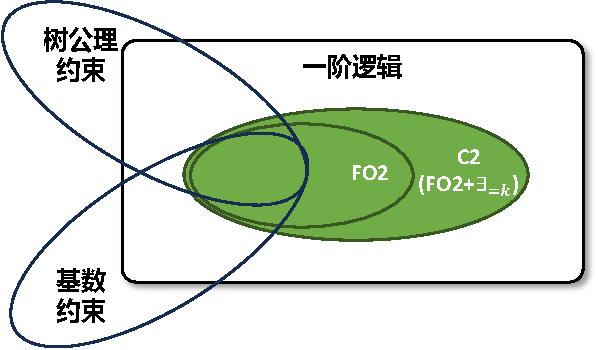
\includegraphics[width=.5\textwidth]{figs/hardness_results.pdf}
  \caption{一阶逻辑模型采样问题已知的复杂度结果}
  \label{fig:hardness_results}
\end{figure}

\subsubsection{1.2.3 公理约束下的一阶逻辑模型计数问题}

实际上,对于如树公理约束的复杂结构约束,WFOMS问题对应的模型计数问题上已存在若干研究\upcite{van_bremen_lifted_2021,toth_lifted_2022,malhotra_lifted_2023}。
相对于WFOMS问题,加权一阶逻辑模型计数(Weighted First-Order Model Counting,WFOMC)问题的目标是计算满足给定一阶逻辑式的模型权重之和。
\cncite{van_bremen_lifted_2021}考虑了树公理约束下的WFOMC问题,证明了\ctwo{}逻辑式中只包含一个树公理约束时,WFOMC问题可以在多项式时间内求解。
\cncite{toth_lifted_2022}证明了在线性序公理约束下,\ctwo{}的WFOMC问题同样可以在多项式时间内求解。
\cncite{malhotra_lifted_2023}将树公理约束的WFOMC算法进一步推广到无环公理约束和弱(强)连通性公理约束上,证明了这些公理约束下的WFOMC问题都存在多项式时间算法。

为了解决上述公理约束下的WFOMC问题,现有工作通常应用对应的组合计数(Enumerative Combinatorics)技术,例如\cncite{van_bremen_lifted_2021}使用基尔霍夫矩阵树定理(Kirchhoff's matrix-tree theorem)来计算树公理约束下的WFOMC问题;组合数学中对连通图和无环图的计数技术被应用到了设计无环公理约束和强(弱)连通性公理约束的WFOMC算法中。
类似的,\cncite{wang_domain-lifted_2019}中为树公理约束设计的WFOMS算法也使用了基尔霍夫矩阵树定理。
显然,这些工作所采用的方法缺乏通用性,一方面难以推广到更为复杂的结构约束,另一方面也无法直接应用于WFOMS算法的设计。

在组合数学中,使用图多项式(Graph Polynomial)对图结构进行计数是一种更为通用的方法\upcite{tutte2004graph,stanley1986enumerative},其中最为著名的是Tutte多项式\upcite{tuttepoly}。
Tutte多项式是一个描述图结构的多项式,其系数可以用来计算图的各种性质,例如生成子图个数、生成树个数等。
Tutte多项式可进一步被推广到有向图\upcite{tutte-directed}。
有向染色多项式(Directed Chromatic Polynomial)\upcite{chromatic-directed}是另一种专门用于有向图的图多项式。
它同样可以用来计算有向图的各种性质,例如强连通分量个数、有向树个数、判断图的无环性等。
因此,相比于使用如基尔霍夫矩阵树定理等特定技术,\emph{使用图多项式技术有望为WFOMS算法的设计提供一种更为通用的方法}。

\subsubsection{1.2.4 一阶逻辑模型采样问题的难解性研究}

\begin{figure}[b]
	\centering
	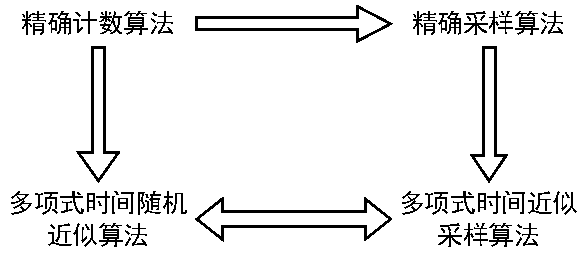
\includegraphics[width=.5\textwidth]{figs/counting_sampling_rel.pdf}
	\caption{加权模型计数和采样问题的等价性}
	\label{fig:counting_sampling_equivalence}
 \end{figure}

对于一阶逻辑模型采样问题的复杂度特征,目前仅有其多项式时间可解性的结果,而对于难解性的分析尚未深入展开。
研究WFOMS问题的难解性除了可以从理论上帮助研究者避免设计无效的算法,另一个关键动机是理论计算机科学领域长期探讨的计数与采样问题的等价性\upcite{jerrum_random_1986}。
 实际上,在给定常量域的情况下,总可以通过实例化(Grounding)过程将一阶逻辑表达式转换为命题逻辑表达式,从而将WFOMC和WFOMS问题转换为命题逻辑中的加权模型计数(Weighted Model Counting,WMC)和WMS问题。
在Leslie Valiant 1986年的工作\cite{jerrum_random_1986}中,WMC和WMS问题理论上的难解性被证明存在一定的等价关系:其精确计数算法、精确采样算法、多项式时间随机近似算法(Fully Polynomial Randomized Approximation Scheme,FPRAS)和多项式时间近似采样算法(Fully Polynomial Approximation Scheme,FPAUS)之间存在如\cref{fig:counting_sampling_equivalence}所示的归约关系\upcite{jerrum_random_1986}。
然而,由于WFOMC和WFOMS问题不具备自还原性\upcite{van_den_broeck_conditioning_2012},是否能将这种对应关系推广到一阶逻辑模型中,仍是一个尚未解决的开放问题。

因此,尽管WFOMC问题已被证明在某些一阶逻辑片段(Fragment)上不存在多项式时间算法\upcite{beame_symmetric_2015,jaeger_lower_2015},但\emph{WFOMS问题的难解性仍然是一个未知问题}。
\cncite{van_den_broeck_conditioning_2012}证明了当一阶逻辑式中允许出现实例化的二元文字(Grounded Binary Literals)时,除非$\#\P=\RP$,否则WFOMC问题不存在多项式时间算法。
\cncite{jaeger_lower_2015}证明了对于一般的一阶逻辑式,除非$\mathsf{ETIME} = \mathsf{NETIME}$,否则WFOMC问题不存在多项式时间(近似)算法。
在\cncite{beame_symmetric_2015}中,该结论被进一步约束到包含三个逻辑变量的一阶逻辑片段\fothree{}上:作者证明了存在一个\fothree{}逻辑式,其WFOMC问题是$\#\P_1$-完全的。
如上所示,WFOMC问题难解性的证明涉及诸如$\#\P$、$\RP$、$\mathsf{ETIME}$、$\mathsf{NETIME}$等复杂性类的假设,使用的证明技术也较为复杂,因此如何将这些结果推广到WFOMS问题上,是一个具有挑战性的问题。

其次,若进一步考虑公理约束,其WFOMC问题的难解性尚且未知,对应的WFOMS问题的难解性分析则更为困难。
观察到一阶逻辑片段上,WFOMC问题难解性与逻辑片段可判定性存在的等价关系,例如\fothree{}逻辑片段是不可判定的\upcite{shoenfield2018mathematical},且WFOMC问题是$\#\P_1$-完全的。
从判定问题的难解性出发,对WFOMS问题的难解性进行分析,可能是一个可行的研究方向。
特别在多个公理约束的不可判定性证明中,如\cncite{charatonik2016two,kieronski_decidability_2013},利用公理约束和一阶逻辑式构造非确定性图灵机(Non-deterministic Turing Machine,NTM)的方法,可以为包含多个公理约束的WFOMS问题难解性分析提供一定的启发。

\subsubsection{1.2.5 一阶逻辑模型采样问题的近似算法设计}

对于WFOMS问题的近似算法设计,主要的工作采用将一阶逻辑式转化为命题逻辑式,然后利用命题逻辑的WMS近似算法来近似求解WFOMS问题的方法。
文献\cite{kukula2000building}基于知识遍历技术,先将逻辑式编译成BDD图,再通过迭代的方法逐步采样各个变量的赋值。
文献\cite{moskewicz2001chaff}采用相似的采样算法,但是基于DPLL的SAT求解器。
同时,也有很多使用马尔可夫链蒙特卡洛方法(Markov Chain Monte Carlo,MCMC)的WMS算法~\upcite{kitchen2010markov,van_den_broeck_lifted_2015,hutchison_new_2005},通常将逻辑式的所有模型看作马尔可夫链的状态,通过转移概率矩阵对模型进行转换,从而使得马尔可夫链的稳态分布达到WMS中定义的分布。
还有一些文献基于概率图模型,将WMS问题反过来转化成一个概率图模型,再使用概率图模型的中的信心传递算法(Belief Propagation)逼近WMS的分布~\upcite{dechter2002generating,gogate2006new}。
上述方法存在的一个主要问题是:当一阶逻辑式转化为命题逻辑式时,会丢失一阶逻辑中重要的\emph{对称性}信息,从而导致转化后的WMS问题规模指数级增长,使得算法的时间复杂度显著增加。

WFOMS问题中的对称性指的是一阶逻辑式的模型具有常量置换不变性,即将逻辑式一个模型中的常量进行任意置换,得到的仍是逻辑式的模型,且这两个模型具有相同的权重。
该性质在多项式时间采样算法的设计中起到了重要作用,例如\cncite{wang_domain-lifted_2019}中提出的WFOMS算法,基于对称性,首先将常量域按照等价类划分,然后通过采样等价类的基数,实现对逻辑式中一元谓词解释(Interpretation)的采样。
目前同样存在一些工作,尝试利用对称性信息设计WFOMS近似算法。
例如,文献\cite{niepert_markov_2012}提出了基于置换轨道(Orbits)的MCMC算法,但没有给出如何计算轨道对应的置换群的方法。
在其后续的研究~\upcite{van_den_broeck_lifted_2015}中,介绍了利用过对称近似(Over-Symmetric Approximation)技巧,先改变原始问题,再使用简单的启发式算法得到原问题的近似对称性,从而得到WFOMS问题中的轨道信息。
文献~\cite{holtzen2020generating}中改进了轨道采样的方法,提出了轨道跳跃(Orbit-Jump)MCMC算法,更一步加速了马尔可夫链的收敛速度。
文献~\cite{DBLP:conf/nips/VenugopalG12}提出了基于分块的Gibbs采样,在该文献中,给出了一个计算最优分块的启发式算法,并给出了Gibbs采样的时间复杂度与分块结果的关系。
上述方法虽然在一定程度上利用了WFOMS问题的对称性,但\emph{忽视了WFOMS问题已有的多项式时间精确采样算法设计,对对称性的分析不够充分}。
例如,\cncite{wang_lifted_2024}中给出的多项式时间精确采样算法基于对称性,将算法分为两步,因此,在设计近似采样算法时,是否可以将这两步分别进行近似,是一个值得进一步研究的问题。

\emph{综上所述,面向结构数据生成的一阶逻辑模型采样问题虽取得了一定的研究进展,但仍存在诸多问题亟待解决。}
\begin{enumerate}
  \item \emph{非有限公理化结构约束下的一阶逻辑模型采样问题}:如何设计支持非有限公理化结构约束的一阶逻辑模型采样算法,是否存在一个类似于图多项式的通用方法,可支持包括树公理约束、无环公理约束、强连通性公理约束等复杂结构约束的一阶逻辑模型采样问题?
  \item \emph{一阶逻辑模型采样问题的难解性分析}:是否所有的一阶逻辑模型采样问题都存在多项式时间算法?如何对一阶逻辑模型采样问题的难解性进行刻画,一阶逻辑片段层面,WFOMS问题的难解性是否存在相变点?
  \item \emph{一阶逻辑模型采样问题的近似算法设计}:如何在一阶逻辑模型采样问题中充分利用对称性信息?是否可以将多项式时间精确采样算法的设计思想应用到近似采样算法设计中?
\end{enumerate}

%对作者个数作了限制以适合申请书
%当作者个数小于等于5个时,予以全部保留,当作者个数大于5个时,只保留3个,加et al
% \newpage
% \bibliographystyle{ieeetrNSFC}

\begin{spacing}{1.1}
{\kaishu \wuhao
\bibliographystyle{GBT7714-2005}
\bibliography{bibs}
}
\end{spacing}
\newpage

\vspace{1.5 \baselineskip}
{\sihao \color{MsBlue} \kaishu 2. {\bfseries 项目的研究内容、研究目标,以及拟解决的关键科学问题}(此部分为重点阐述内容);}

% 2.1 研究目标
\subsection{2.1 研究内容}

针对当前一阶逻辑模型采样问题的研究现状和存在的问题,本项目拟从\emph{``结合图多项式的一阶逻辑模型采样算法''}、\emph{``一阶逻辑模型采样问题的难解性分析''}以及\emph{``基于对称性的一阶逻辑模型采样近似算法设计''}三个方面展开研究,具体研究内容如下,如\cref{fig:content}所示。
其中,\emph{研究内容一}旨在解决一阶逻辑模型采样问题中对非有限公理化结构约束的支持问题,通过引入图多项式等代数图论工具,设计支持包括树公理约束、森林公理约束、$k$-弱连通公理约束等弱连通性约束,以及包括强通公理约束、无环公理约束等强连通性约束的一阶逻辑模型精确采样算法;
\emph{研究内容二}对一阶逻辑模型采样问题的难解性进行深入分析,研究一阶逻辑模型采样问题在不同逻辑片段上,包含全一阶逻辑和\fothree{}逻辑片段,以及更一般的包含二元关系和多个公理约束上的难解性,旨在揭示从可解的\fotwo{}逻辑片段到一般情况下,一阶逻辑模型采样问题的复杂度相变性质;
\emph{研究内容三}在研究内容一和研究内容二的基础上,设计基于对称性的一阶逻辑模型采样近似算法,通过深入分析精确采样算法的设计思想,为难解的一阶逻辑模型采样问题设计高效的近似采样算法。


\begin{figure}[H]
  \centering
  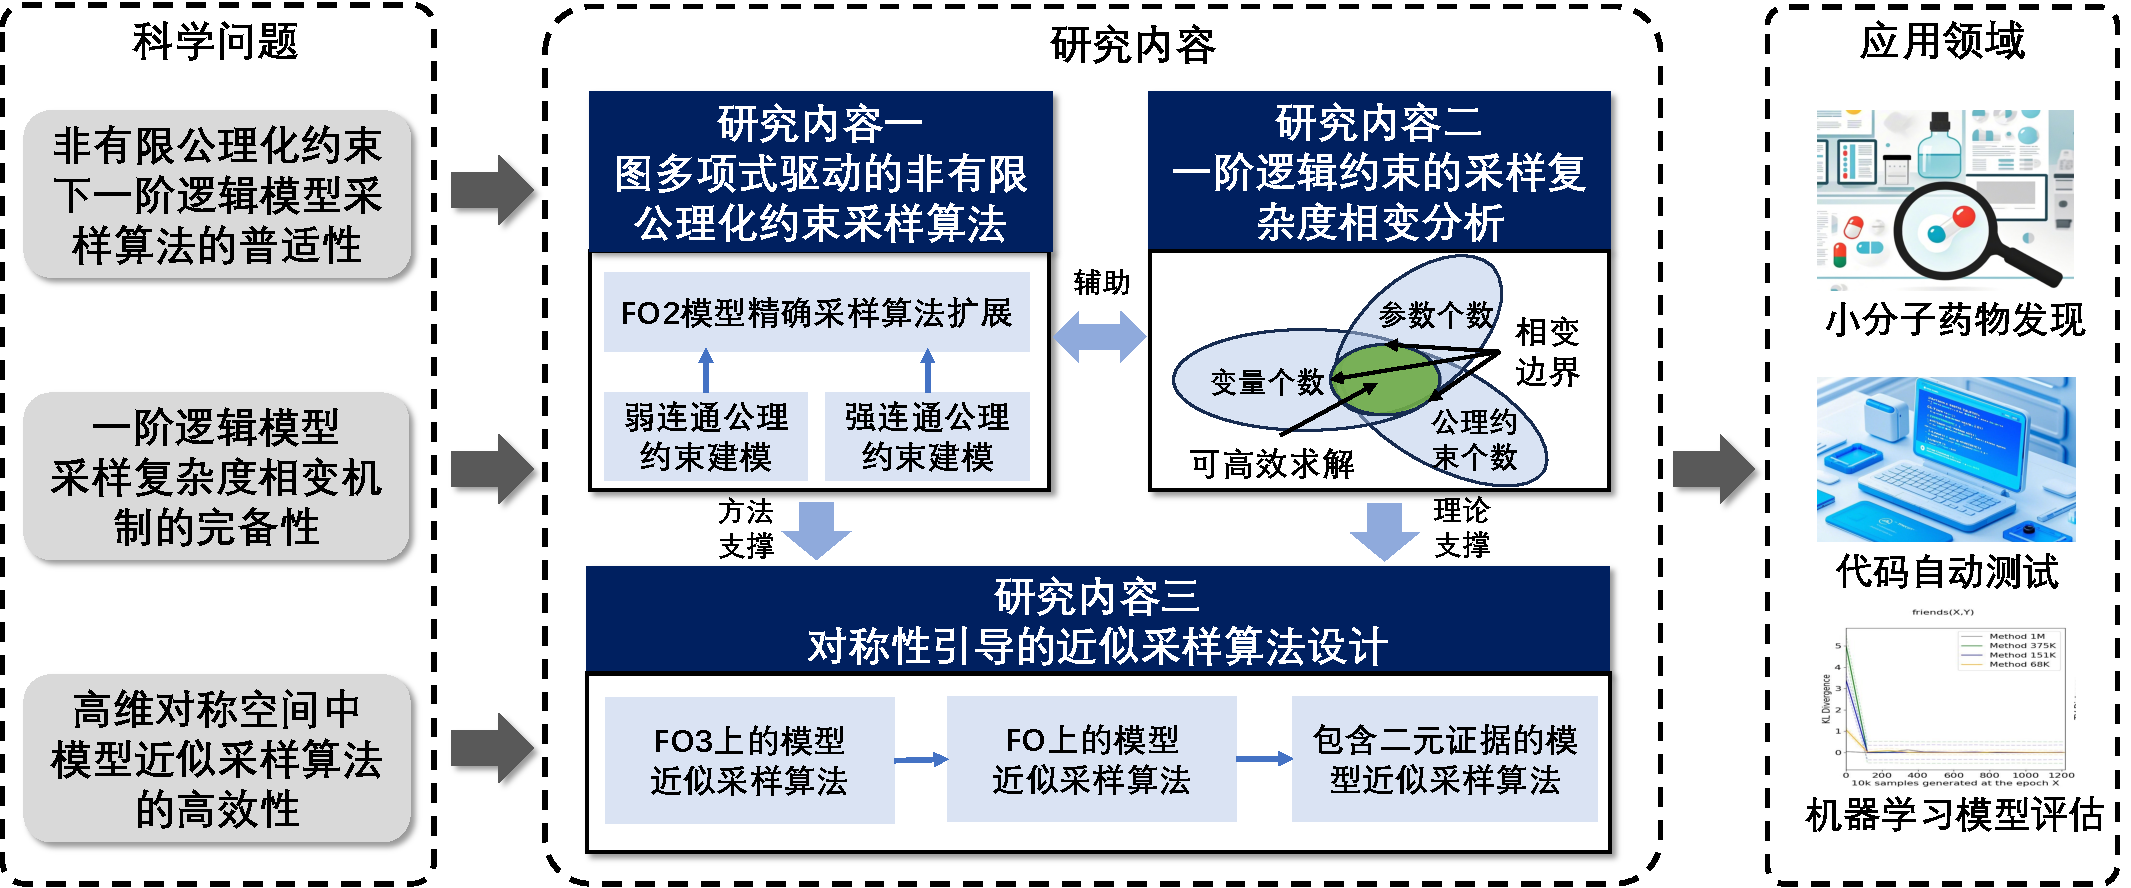
\includegraphics[width=\textwidth]{figs/content.pdf}
  \caption{研究内容分解图}
  \label{fig:content}
\end{figure}

\textbf{研究内容一:结合图多项式的一阶逻辑模型采样算法设计}

本项目结合图多项式工具,设计非有限公理化结构约束下的一阶逻辑模型采样的统一算法框架。
该部分研究内容主要包括:首先,深入分析典型的图多项式(包括Tutte多项式、有向染色多项式)在组合计数中的应用,以及完全图和分块图上图多项式的计算方法;其次,利用一阶逻辑语言对图多项式进行形式化描述,对于Tutte多项式和有向染色多项式,构建对应的一阶逻辑模型采样问题,实现对包括树公理约束、森林公理约束、$k$-弱连通公理约束、强通公理约束、无环公理约束等公理约束的统一建模;最后,针对结合图多项式的一阶逻辑模型采样问题,设计多项式时间精确采样算法,实现上述公理约束下高效的模型采样。

\textbf{研究内容二:一阶逻辑模型采样问题的难解性分析}

本项目研究多种形式下一阶逻辑模型采样问题的难解性,包括全一阶逻辑模型采样问题、\fothree{}逻辑片段上的模型采样问题、以及包含二元关系的一阶逻辑模型采样问题和包含多个公理约束的一阶逻辑模型采样问题。
该部分研究内容主要包括:首先,通过分析一阶逻辑模型计数问题难解性和一阶逻辑不可判定性的证明,得到与一阶逻辑模型采样问题相关的难解问题,如一阶逻辑的谱问题,命题逻辑上模型采样问题、平铺问题(Tiling Problem)等;其次,通过构造适当的约化,或通过直接使用一阶逻辑构造非确定性图灵机,证明一阶逻辑模型采样问题在不同逻辑片段上的难解性,揭示难解性的相变性质;最后,将难解性结果推广到更一般的包含二元关系和多个公理约束的一阶逻辑模型采样问题上,进一步完善一阶逻辑模型采样问题的复杂度理论。

\textbf{研究内容三:基于对称性的一阶逻辑模型采样近似算法设计}

本项目研究基于一阶逻辑模型精确采样算法中对对称性的分析,设计高效的近似采样算法。
该部分研究内容主要包括:首先,针对\fothree{}逻辑片段,由\fotwo{}精确采样算法中分步采样的思想,研究当逻辑式中只包含全称量词时的近似采样算法设计,对精确算法中第二步采样步骤进行并行化,提高近似采样算法的效率;
其次,基于全一阶逻辑上模型采样问题的对称性,探索基于谓词基数分块的近似采样算法设计,通过先采样谓词基数,再在谓词基数的约束下采样谓词解释,实现全一阶逻辑上高效的模型近似采样。
最后,研究包含二元证据的\fotwo{}逻辑片段上的WFOMS问题,同样由精确采样算法的设计思想,采用第一步近似采样、第二步精确采样的方法,设计高效的近似采样算法;

% 2.2 研究内容
\subsubsection{2.2 研究目标}

\begin{itemize}
  \item 一阶逻辑模型采样的通用算法设计,支持包含公理约束的一阶逻辑模型采样问题;
  \item 一阶逻辑模型采样问题的难解性分析,揭示一阶逻辑模型采样复杂度的二分性质;
  \item 针对难解的一阶逻辑模型采样问题,设计高效的近似采样算法。
\end{itemize}

% 2.3 拟解决的关键科学问题
\subsubsection{2.3 拟解决的关键科学问题}

\begin{itemize}
  \item 公理约束的统一建模问题;
  \item 一元语言的图灵机建模问题;
  \item 近似采样算法中实体对称性的利用问题;
\end{itemize}


\newpage

{\sihao \color{MsBlue} \kaishu 3.{\bfseries 拟采取的研究方案及可行性分析} (包括研究方法、技术路线、实验手段、关键技术等说明);}

% 3.1 拟采取的技术路线
\subsection{3.1 拟采取的研究方案}

本项目针对一阶逻辑模型采样问题,在申请人已有相关研究成果的基础上,围绕``结合图多项式的一阶逻辑模型采样算法''、``一阶逻辑模型采样问题的难解性分析''和``基于对称性的一阶逻辑模型采样近似算法设计''三个方面展开研究。
具体拟采取的研究方案如下,如\cref{fig:plan}所示。
首先,通过将图多项式引入到一阶逻辑模型采样问题中,定义一阶逻辑上的弱连通多项式、非严格强连通多项式和严格强连通多项式,实现对公理约束的统一建模,并在此基础上设计公理约束下的多项式时间模型采样算法;
其次,通过一阶逻辑的谱问题、网格公理约束下的谱问题以及$\#2$-CNF问题的归约,分别证明全一阶逻辑、\fothree{}逻辑片段上、以及包含二元证据和多个公理约束的一阶逻辑模型采样问题的难解性;
最后,基于对称性的分析,针对\fothree{}逻辑片段、全一阶逻辑以及包含二元证据的\fotwo{}逻辑片段,分别设计并行化采样、基于谓词基数分块和基于分块吉布斯采样的近似采样算法。



\begin{figure}[H]
  \centering
  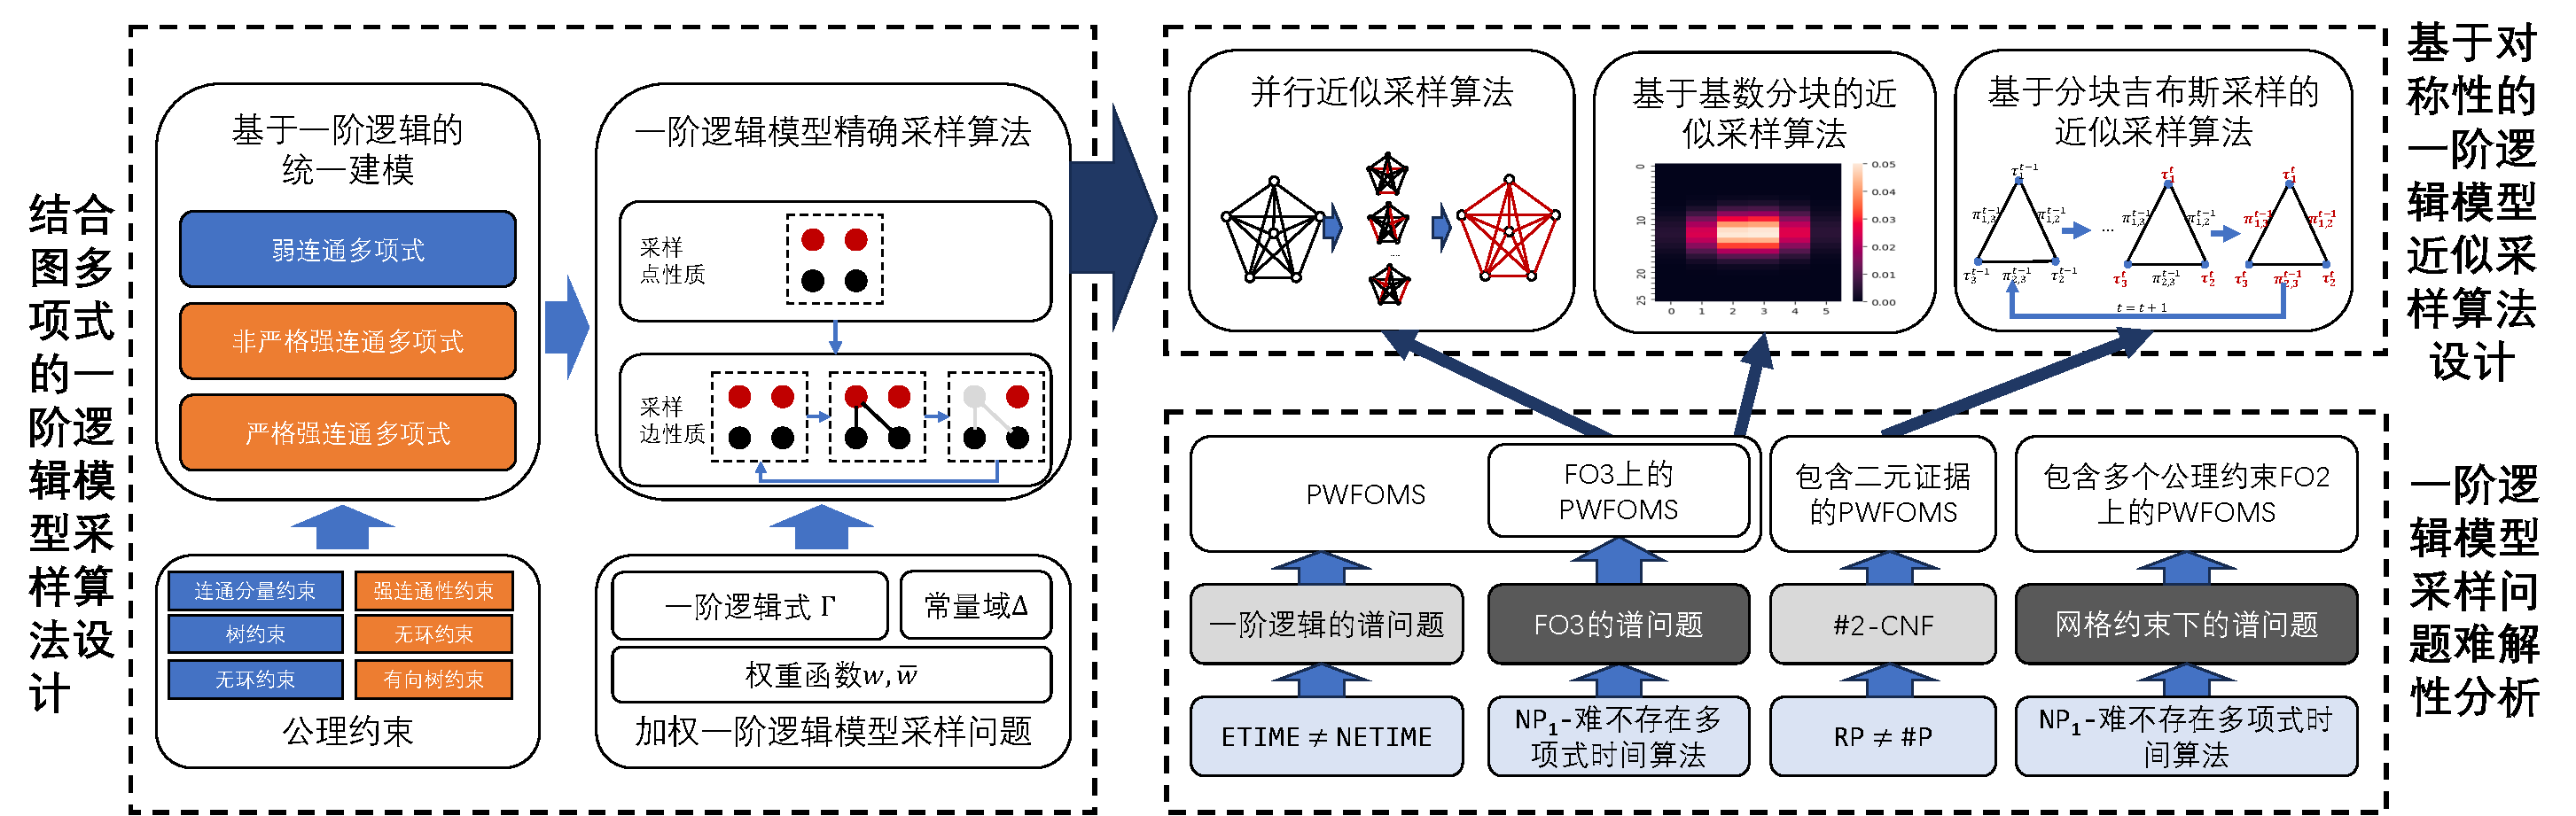
\includegraphics[width=\textwidth]{figs/plan.pdf}
  \caption{拟采取的研究方案}
  \label{fig:plan}
\end{figure}

\subsubsection{3.1.1 结合图多项式的一阶逻辑模型采样算法设计}

% 受到代数图论中使用图多项式(Graph Polynomial)对组合计数(Enumerative Combinatorics)问题进行研究的启发,本部分拟设计一种结合图多项式的一阶逻辑模型采样算法。
% 在代数图论中,图多项式是一种用于描述图结构的不变量,一个图的各种结构特征可以通过其图多项式的系数来表示,例如在Tutte多项式中,图的生成森林(Spanning Forest)、无环定向(Acyclic Orientation)个数对应度数为$(1,1)$和$(2,0)$的项的系数,从而通过计算图多项式,可以得到图的各种结构特征。

受到代数图论中使用图多项式(Graph Polynomial)对组合计数(Enumerative Combinatorics)问题进行研究的启发,本部分拟设计一种结合图多项式的一阶逻辑模型采样算法。
首先,发现某些图多项式的计算问题可以使用一阶逻辑进行形式化描述,例如,Tutte多项式可以被形式化的定义为一元谓词在弱连通子图上的传递关系(见\cref{def:wcp})。
从而一系列的结构公理约束,例如弱连通性约束、树约束等,可以被一阶逻辑上对应的多项式统一建模。
如\cref{tab:axioms}所示,分别结合Tutte多项式和有向染色多项式,定义了一阶逻辑上的弱连通多项式和强连通多项式,实现了对一系列公理约束的统一建模。
这些公理约束下的一阶逻辑模型采样问题可以归约为弱连通多项式和强连通多项式的计算问题,从而得到公理约束下一阶逻辑模型采样问题的高效求解算法。
本部分采用的技术路线如\cref{fig:polynomial}所示,先对于弱连通性公理和强连通性公理,分别定义了对应的弱连通多项式和强连通多项式,然后通过对已有的\fotwo{}模型采样算法进行扩展,进行基于弱连通多项式和强连通多项式的一阶逻辑模型采样算法设计。

\begin{figure}[t]
  \centering
  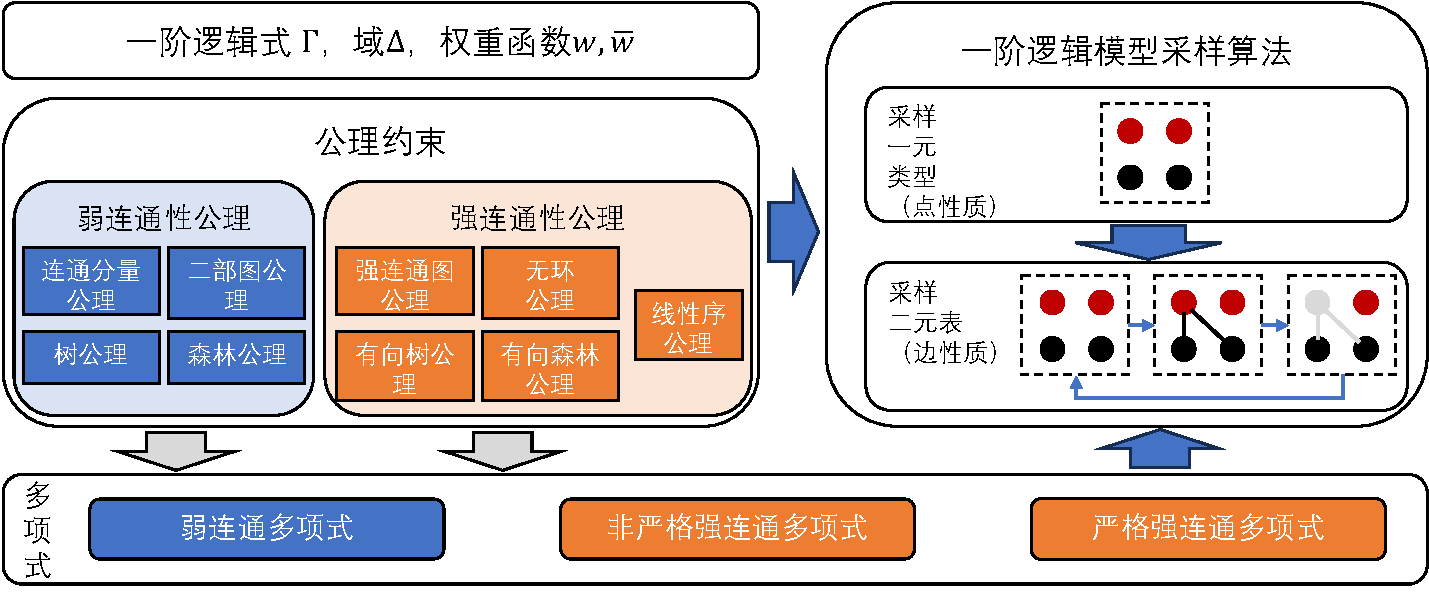
\includegraphics[width=\textwidth]{figs/polynomial.pdf}
  \caption{结合图多项式的一阶逻辑模型采样算法设计技术路线}
  \label{fig:polynomial}
\end{figure}

\begin{table}[h]
  \centering
  \caption{基于图多项式的公理约束统一建模方法}\label{tab:axioms}
    \begin{tabular}{l|l|l}
      \hline
      \textbf{公理约束} & \textbf{描述} & \textbf{建模方法} \\
      \hline\hline
      $connected_k(R)$ & $G(R)$中存在$k$个连通分量 & 弱连通多项式 \\
      \hline
      $bipartite(R)$ & $G(R)$是二分图 & 弱连通多项式 \\
      \hline
      $tree(R)$ & $G(R)$是树 & 弱连通多项式 \\
      \hline
      $forest(R)$ & $G(R)$是森林 & 弱连通多项式 \\
      \hline\hline
      $SC(R)$ & $G(R)$是强连通图 & 非严格强连通多项式 \\
      \hline
      $AC(R)$ & $G(R)$是无环图 & 严格强连通多项式 \\
      \hline
      $DT(R, Root)$ & $G(R)$是以$Root$为根的有向树 & 非严格强连通多项式 \\ \hline
      $DF(R)$ & $G(R)$是有向森林 & 非严格强连通多项式 \\ \hline
      $LO(R)$ & $R$表示线性序关系 & 非严格强连通多项式 \\
      \hline
    \end{tabular}
\end{table}

\subsubsubsection{(1)一阶逻辑模型采样问题}

本项目关注纯关系(Pure Relation)的一阶逻辑,即不包含函数符号。
该类一阶逻辑包含一个无限的逻辑变量符号集合和一个有限的谓词符号集合。
谓词的元数表示该谓词的参数个数,一般将一个谓词记作$P/k$,其中$P$是谓词的名称,$k$是谓词的元数。
如果$R$是一个元数为$k$的谓词符号,$x_1,\dots,x_k$是$k$个逻辑变量,则$R(x_1,\dots,x_k)$是一个原子式。
一阶逻辑中的文字定义为一个原子式或其否定。
一阶逻辑式可以是一个文字(Literal),或者两个一阶逻辑式的合取或析取。
除此之外,一阶逻辑还允许使用全称量词$\forall$和存在量词$\exists$,对逻辑变量进行约束,被量词约束的一阶逻辑式仍然是一个一阶逻辑式。
无自由变量的一阶逻辑式,被称作一阶逻辑语句。
给定一组谓词$\mathcal{P}$,一个$\mathcal{P}$-结构为一个元组$(\domain, \mathcal{I})$,其中$\domain$是一个非空常量集合,称为域(Domain),$\mathcal{I}$是一个函数,将$\mathcal{P}$中的每个谓词符号$P_i/k_i$映射到$\domain^{k_i}$的一个子集,代表$P_i$为真的赋值;$\mathcal{I}(P_i)$称为$P_i$的解释(Interpretation)。
将一阶逻辑式$\formula$中的谓词集合记作$\mathcal{P}_\formula$,则$\formula$的结构定义为一个$\mathcal{P}_\formula$-结构。
一个结构$\structure=(\domain, \mathcal{I})$满足包含全称量词的一阶逻辑式$\forall x: \phi(x)$,当且仅当将$\phi(x)$中的自由变量$x$替换为$\domain$中的任意常量后,$\structure$满足替换后的一阶逻辑式;结构$\structure$满足包含存在量词的一阶逻辑式$\exists x: \phi(x)$,当且仅当存在$\domain$中的某个常量,将$\phi(x)$中的自由变量$x$替换为该常量后,$\structure$满足替换后的一阶逻辑式。
若结构$\structure$满足一阶逻辑式$\formula$,则称$\structure$是$\formula$的一个模型,表示为$\structure\models\formula$。
给定一个一阶逻辑式$\formula$和一个域$\domain$,使用$\fomodels{\formula}{\domain}$表示$\formula$在$\domain$上的所有模型的集合。


一阶逻辑模型计数问题的目标是计算$\fomodels{\formula}{\domain}$的大小,即$\sentence$在$\domain$上的模型个数;一阶逻辑模型采样问题则从$\fomodels{\formula}{\domain}$中均匀随机采样一个模型。

\begin{definition}[一阶逻辑模型采样问题\upcite{wang_domain-lifted_2019,wang_exact_2023-1,wang_lifted_2024}]
	一阶逻辑语句$\sentence$在域$\domain$上的一阶逻辑模型采样问题(FOMS)是从$\fomodels{\sentence}{\domain}$中均匀随机采样一个模型,即对任意$\mu\in\fomodels{\sentence}{\domain}$,输出$\mu$的概率为 $\pro[\mu]=1/|\fomodels{\sentence}{\domain}|$.
\end{definition}
加权一阶逻辑模型采样问题在FOMS的基础上,引入了一组额外的加权函数$(\weight, \negweight)$,它们将$\sentence$中的所有谓词映射到一组权重:$\mathcal{P}_\sentence \to \real$。
基于这组加权函数,可以定义一个文字集合的权重。
\begin{definition}[文字集合的权重]
	\label{def:weight-of-literals}
	给定一组加权函数$(\weight, \negweight)$和一个文字集合$L$,在$(\weight, \negweight)$下,$L$的权重定义为
	\begin{equation}
		\typeweight{L} := \prod_{l\in L_T}\weight(\mathsf{pred}(l)) \cdot \prod_{l\in L_F}\negweight(\mathsf{pred}(l))
	\end{equation}
其中$L_T$(或$L_F$)表示$L$中为真(或假)的文字的集合,$\mathsf{pred}(l)$将一个文字$l$映射到其对应的谓词名称。
\end{definition}

给定一个一阶逻辑语句$\sentence$和一个域$\domain$,$\sentence$在$\domain$上的任意一个结构$\structure$都可以看作是一个文字的集合,集合中的文字是否为真,由$\structure$中的解释决定,因此可以将一个结构的权重定义为其对应文字集合的权重。

\begin{definition}[加权一阶逻辑模型计数问题\upcite{beame_symmetric_2015}]\label{def:wfomc}
	给定一个一阶逻辑语句$\sentence$、$\sentence$上的一组权重函数$(\weight, \negweight)$及一个域$\domain$,则$\sentence$在域$\domain$和$(\weight, \negweight)$下的加权一阶逻辑模型计数问题(\wfomc)为$\symwfomc(\sentence, \domain, \weight, \negweight) := \sum_{\mu\in\fomodels{\sentence}{\domain}}\typeweight{\mu}$。
\end{definition}
\begin{definition}[加权一阶逻辑模型采样问题\upcite{wang_lifted_2024,wang_exact_2023-1,wang_domain-lifted_2019}]
\label{def:wfoms}
	给定一个一阶逻辑语句$\sentence$、一组从$\sentence$中谓词到非负实数的权重函数$(\weight, \negweight)$:$\mathcal{P}_\sentence\to\real_{\ge 0}$及一个域$\domain$,则$\sentence$在域$\domain$和$(\weight, \negweight)$下的加权一阶逻辑模型采样问题(WFOMS)定义为:随机生成$\fomodels{\sentence}{\domain}$中的一个模型$\mu$,使得其生成的概率为$\pro[\mu] = \typeweight{\mu}/\symwfomc(\sentence, \domain, \weight, \negweight)$。
	% 其中$\typeweight{\mu}$是模型$\mu$的权重。
\end{definition}

给定一个二元谓词$R/2$,$R$的一个解释$\mathcal{I}(R)$可以看作是一个有向图,记为$G(R)$,其中域$\domain$表示图的顶点集,$R$的解释$\mathcal{I}(R)$表示图的边集。
给定一个结构$\structure$,记$R$的解释$\structure_R$表示的图为$G(\structure_R)$。
\emph{公理约束(axiom)}是对二元谓词$R$的解释$G(R)$的一种特殊约束,要求$G(R)$满足某种特定的结构。
例如,树公理要求$G(R)$是一棵树,森林公理要求$G(R)$是一个森林。
通常可以将公理约束写作$axiom(R)$的形式,其中$axiom$表示公理的名称,$R$表示公理约束作用的谓词。
例如,$tree(E) \land \forall x \left( Leaf(x)\leftrightarrow \exists_{=1} y \ E(x,y) \right)$约束$E$是一棵树,其中$Leaf$表示叶子节点。
包含公理约束的一阶逻辑模型计数和采样问题是一种特殊的加权一阶逻辑模型计数和采样问题,其定义与\cref{def:wfomc,def:wfoms}类似,只是在计数和采样的过程中,需要额外考虑公理约束的约束条件。

\subsubsubsection{(2)基于Tutte多项式的弱连通性公理约束统一建模}

首先考虑弱连通性公理约束的统一建模问题,包括树公理、森林公理、$k$-连通性公理等。
本项目拟基于Tutte多项式的概念,对弱连通性公理约束进行统一建模。
% Tutte多项式是图论中的一个重要概念,它是图的一个不变量,可以用来描述图的各种性质。
% 考虑一个无向图$G=(V,E)$,其中$V$是顶点集合,$E$是边集合。
% 图$G$的Tutte多项式$T_G(x,y)$是一个关于$x$和$y$的多项式,定义为
% \begin{equation*}
% T_G(x,y) = \sum_{A \subseteq E} (x-1)^{cc(A)-cc(E)} (y-1)^{cc(A)+|A|-|V|}
% \end{equation*}
% 其中$cc(E)$是图$G$的边的连通分量的数量,$cc(A)$是只考虑$A$中的边的情况下图$G$的边的连通分量的数量。
% Tutte多项式具有重要的组合学意义。在特定点处求解多项式可以揭示各种组合学性质。例如,$T_G(1,1)$计算图$G$的生成树数量(如果$G$是连通的,则是生成树的数量);$T_G(0,2)$计算图$G$的强连通有向图的数量。
% 同时,只替换一个变量的具体值,就可以得到图$G$的其他多项式。例如,$T_G(x,0)$是图$G$的色多项式(Chromatic Polynomial),$T_G(0,y)$是图$G$的流多项式(Flow Polynomial)。
基于Tutte多项式的概念,本项目拟通过将Tutte多项式在各特定点处的值表示成一个一阶逻辑式,从而实现对弱连通性公理约束的统一建模。
具体来说,定义\emph{弱连通多项式}如下。

\begin{definition}[弱连通多项式]\label{def:wcp}
  令$\Psi$为一个一阶逻辑语句,$\weight, \negweight$为加权函数,$R$为一个二元关系。
  $\Psi$的$n$阶弱连通多项式$f_n(u)$定义为满足以下条件的一元多项式:
  \begin{equation*}
  f_n(u;\Psi, \weight, \negweight, R) = \symwfomc(\Psi_{R,u}, n, \weight, \negweight).
  \end{equation*}
  其中$\Psi_{R,u}$是一个一阶逻辑语句,定义如下:
  \begin{equation}
    \begin{aligned}
      \Psi_{R,u} = \Psi \wedge & \bigwedge_{i=1}^u \forall x \forall y \left( A_i(x) \wedge (R(x,y) \vee R(y,x)) \to A_i(y) \right) \\
      \wedge & \bigwedge_{i = 2}^u \forall x \left( A_i(x) \to A_{i-1}(x) \right)
    \end{aligned}
    \label{eq:wcp}
  \end{equation}
  这里$A_1, \dots, A_u$是$u$个新的一元谓词,$w(A_i) = \overline{w}(A_i) = 1$。
\end{definition}

直觉上,通过引入$u$个新的谓词$A_1, \dots, A_u$,每个弱连通分量在$G(R)$中对应的顶点集合都会被标记为相同的$A_i$,从而使得每个弱连通分量对\wfomc{}的贡献为$u+1$。
令$cc(\mu_R)$表示$G(\mu_R)$中的弱连通分量的数量,下面的命题表明弱连通多项式$f_n(u)$与$cc(\mu_R)$之间的关系。

\begin{proposition}\label{prop:wcp}
  任意一阶逻辑语句$\Psi$的$n$阶弱连通多项式$f_n(u)$满足
  \begin{equation*}
    f_n(u;\Psi, \weight, \negweight, R) = \sum_{\mu \in \fomodels{\Psi}{n}} \typeweight{\mu} \cdot (u+1)^{cc(\mu_R)}
  \end{equation*}
\end{proposition}

通过\cref{prop:wcp},可以将公理约束$axiom(R)$的约束条件建模为弱连通多项式$f_n(u)$系数的约束条件,从而实现对弱连通性公理约束的统一建模。
令$[u^k] f_n(u)$表示多项式$f_n(u)$中$u^k$的系数。

\paragraph{$k$-连通性约束} $k$-连通性约束$connected_k(R)$要求$G(R)$是一个$k$-连通图,即$G(R)$中包含$k$个弱连通分量。
利用弱连通多项式$f_n(u)$,可以将$k$-连通性约束建模为$f_n(u)$中$u^k$的系数约束:$\symwfomc(\Psi \land connected_k(R), n, \weight, \negweight) = [u^k] f_n(u - 1; \Psi, \weight, \negweight, R)$。

\paragraph{树公理约束} 树公理约束$tree(R)$要求$G(R)$是一棵树,即$G(R)$中包含$cc(\mu_R) = 1$个弱连通分量,且$G(R)$中的边数为$n-1$。
定义拓展的弱连通多项式$f_n(u,v)$为
\begin{equation*}
  f_n(u, v; \Psi, \weight, \negweight, R) = \symwfomc(\Psi_{R,u}, n, \weight_{R,v}, \negweight)
\end{equation*}
其中$\weight_{R,v}(R) = \weight(R) \cdot v$。
利用拓展的弱连通多项式$f_n(u,v)$,可以将树公理约束建模为$f_n(u,v)$中$uv^{n-1}$的系数约束:$\symwfomc(\Psi \land tree(R), n, \weight, \negweight) = [uv^{2(n-1)} ] f_n(u-1, v; \Psi, \weight, \negweight, R)$。

\paragraph{森林公理约束} 森林公理约束$forest(R)$要求$G(R)$是一个森林,即$G(R)$中包含$cc(\mu_R)$个弱连通分量,且$G(R)$中的边数为$n - cc(\mu_R)$。
类似于树公理约束,利用拓展的弱连通多项式$f_n(u,v)$,可以将森林公理约束建模为$f_n(u,v)$中$u^{cc(\mu_R)}v^{n-cc(\mu_R)}$的系数约束:$\symwfomc(\Psi \land forest(R), n, \weight, \negweight) = \sum_{i=1}^n [u^iv^{2(n-i)}] f_n(u-1, v; \Psi, \weight, \negweight, R)$。

\paragraph{二部图公理约束}
二部图公理约束$bipartite(R)$要求$G(R)$是一个二部图,即$G(R)$中的顶点可以被分为两个不相交的集合$V_1$和$V_2$,使得$R$只连接$V_1$和$V_2$中的顶点。
令
\begin{align*}
  \sentence_b = &\symsentence \land \forall x \ ((P_1(x) \lor P_2(x)) \land (\lnot P_1(x) \lor \lnot P_2(x))) \\
    &\land \forall x \forall y \ \left( P_1(x) \land P_1(y) \lor P_2(x) \land P_2(y) \to \lnot R(x,y) \right)
\end{align*}
其中,$P_1, P_2$是新的一元谓词,将顶点集合分为两个不相交的集合。
则二部图公理约束可以建模为
\begin{align*}
  \symwfomc(\sentence \land bipartite(R), n, \weight, \negweight) &= \sum_{\mu\in\fomodels{\sentence_b}{n}} \typeweight{\mu}\cdot (\frac{1}{2})^{cc(\mu_R)} \\
  &= f_n(-\frac 12; \sentence_b, \weight, \negweight, R)
\end{align*}
上式中每个模型的权重需要乘以$(\frac{1}{2})^{cc(\mu_R)}$,因为对于二部图中的每个连通分量,$P_1$和$P_2$可以交换位置,从而导致了重复计数。

利用弱连通多项式$f_n(u)$,不仅可以对于严格的公理约束进行建模,还可以建模更为复杂的软约束。例如,在一个社交网络中,可以通过$G(friends)$中的连通分量的数量来表示紧密度,即连通分量的数量越少,网络越紧密。
在这种情况下,可以将一个实数$d$用来表示紧密度:$d$越大,网络越紧密,即$G(friends)$中的连通分量数量越少。
这可以通过定义模型$\mu$的权重为$\typeweight{\mu}\cdot \exp(-d\cdot cc(\mu_{friends}))$来实现,
那么社交网络的生成问题即对应着$f_n(\exp(-d) - 1; \sentence, \weight, \negweight, friends)$上的模型采样问题。

\subsubsubsection{(3)基于有向染色多项式的强连通公理约束统一建模}

该部分拟基于有向染色多项式(Directed Chromatic Polynomial)的概念,对强连通公理约束,例如强连通分量公理约束、无环公理约束等,进行统一建模。
% 有向染色也是图论中的一个重要概念,它是有向图的一个不变量,可以用来描述有向图的各种性质。
% 给定一个有向图$D=(V,E)$,其中$V$是顶点集合,$E$是边集合。

使用$\chi_D(x)$表示有向图$D$的严格有向染色多项式(Strict Directed Chromatic Polynomial),定义为将$V$中的顶点用$\{1, 2, \dots, x\}$中的颜色染色,使得如果有一条从$u$到$v$的边,则$u$的颜色\emph{小于}$v$的颜色的染色方案的数量。
易知$\chi_D(x)$是一个关于$x$的多项式,且$\chi_D(x)$的次数为$|V|$。
类似地,使用$\bar \chi_D(x)$表示有向图$D$的非严格有向染色多项式(Non-Strict Directed Chromatic Polynomial),定义为将$V$中的顶点用$\{1, 2, \dots, x\}$中的颜色染色,使得如果有一条从$u$到$v$的边,则$u$的颜色\emph{小于等于}$v$的颜色的染色方案的数量。
同样,$\bar \chi_D(x)$是一个关于$x$的多项式,且$\bar \chi_D(x)$的次数为$|V|$。
令$acyc(D)$表示将有向图$D$中的所有环压缩后得到的无环有向图,则严格有向染色多项式和非严格有向染色多项式之间有如下关系:
\begin{equation*}
\begin{aligned}
\chi_D(x) &= \begin{cases}
    (-1)^n \bar \chi_D(-x), & D \text{ is acyclic,} \\
    0, & \text{otherwise}
    \end{cases} \\
\bar \chi_D(x) &= (-1)^{|V(acyc(D))|} \chi_{acyc(D)}(-x)
\end{aligned}
\end{equation*}

\begin{definition}[强连通多项式]\label{def:scp}
  令$\Psi$为一个一阶逻辑语句,$\weight, \negweight$为权重函数,$R$为一个二元关系。
  $\Psi$的$n$阶\emph{严格强连通多项式}定义为满足以下条件的二元多项式:
  \begin{equation*}
  g_n(u,v;\Psi, \weight, \negweight, R) = \symwfomc(\Psi_{R,u,v}, n, \weight, \negweight)
  \end{equation*}
  其中$\Psi_{R,u,v}$是一个一阶逻辑语句,定义如下:
  \begin{equation}
  \begin{aligned}
    \sentence \land & \bigwedge_{i=1}^u \forall x \forall y \left( A_i(x) \wedge (R(x,y) \vee R(y,x)) \to A_i(y) \right) \\
    \wedge & \bigwedge_{i = 2}^u \forall x \left( A_i(x) \to A_{i-1}(x) \right) \wedge \bigwedge_{i=1}^{v-1} \forall x \forall y \left( B_i(x) \wedge R(x,y) \to B_{i+1}(y) \right) \\
    \wedge & \forall x \forall y \left( R(x,y) \to \lnot B_v(x) \land B_1(y) \right) \wedge \bigwedge_{i = 2}^v \forall x \left( B_i(x) \to B_{i-1}(x) \right)
\end{aligned}
\label{eq:sscp}
  \end{equation}
  这里$A_1, \dots, A_u$和$B_1, \dots, B_v$是$u$个和$v$个新的一元谓词。
  类似的,定义$n$阶\emph{非严格强连通多项式}为
  \begin{equation*}
  \bar g_n(u,v;\Psi, \weight, \negweight, R) = \symwfomc(\bar \Psi_{R,u,v}, n, \weight, \negweight),
  \end{equation*}
  其中$\bar \Psi_{R,u,v}$是一个一阶逻辑语句,定义如下:
  \begin{equation}
    \begin{aligned}
      \sentence \land & \bigwedge_{i=1}^u \forall x \forall y \left( A_i(x) \wedge (R(x,y) \vee R(y,x)) \to A_i(y) \right) \wedge \bigwedge_{i = 2}^u \forall x \left( A_i(x) \to A_{i-1}(x) \right)\\
      \wedge & \bigwedge_{i=1}^v \forall x \forall y \left( B_i(x) \wedge R(x,y) \to B_i(y) \right) \wedge \bigwedge_{i = 2}^v \forall x \left( B_i(x) \to B_{i-1}(x) \right)
    \end{aligned}
    \label{eq:nscp}
  \end{equation}
\end{definition}

从上述定义中可以看出,$A_1, \dots, A_u$主要用于捕获$G(R)$的弱连通分量的信息,而$B_1, \dots, B_v$主要用于捕获$G(R)$中边的方向性,从而使得$R$的强连通性得到约束。
类似弱连通多项式,强连通多项式和的系数与$cc(\mu_R)$以及$G(\mu_R)$的有向染色多项式之间有如下关系。
\begin{proposition}\label{prop:scp}
  一阶逻辑语句$\Psi$的$n$阶严格强连通多项式和非严格强连通多项式满足
  \begin{align*}
  g_n(u,v;\Psi, \weight, \negweight, R) &= \sum_{\mu \in \fomodels{\Psi}{n}} \typeweight{\mu} \cdot (u+1)^{cc(\mu_R)} \cdot \chi_{G(\mu_R)}(v+1) \\
  \bar g_n(u,v;\Psi, \weight, \negweight, R) &= \sum_{\mu \in \fomodels{\Psi}{n}} \typeweight{\mu} \cdot (u+1)^{cc(\mu_R)} \cdot \bar \chi_{G(\mu_R)}(v+1)
  \end{align*}
\end{proposition}
由上述命题和严格有向染色多项式及非严格有向染色多项式的性质,可知$g_n(u,v;\linebreak \Psi, \weight, \negweight, R)$和$\bar g_n(u,v;\Psi, \weight, \negweight, R)$是关于$u$和$v$的二元多项式,且二元多项式的次数不超过$n$。

利用强连通多项式,可以对于强连通性公理约束进行建模。
\paragraph{强连通分量公理约束} 强连通分量公理约束$SC(R)$要求$G(R)$是一个强连通图,即$G(R)$中包含一个强连通分量。可以将强连通分量公理约束建模为
\begin{align*}
    -[u]\bar g_{n}(u-1, -2; \sentence, \weight, \negweight, R)
    =& -[u]\sum_{\mu \in \fomodels{\Psi}{n}} \typeweight{\mu} \cdot u^{cc(\mu_R)} \cdot \bar \chi_{G(\mu_R)}(-1) \\
    =& -\sum_{\substack{\mu \in \fomodels{\sentence}{n}: \\ G(\mu_R)\text{ is strongly connected}}} -\typeweight{\mu} \\
    =& \symwfomc(\sentence \land SC(R), n, \weight, \negweight)
\end{align*}

\paragraph{无环公理约束} 无环公理约束$AC(R)$要求$G(R)$是一个无环图,即$G(R)$是一个有向无环图。可以将无环公理约束建模为$(-1)^n \cdot g_{n}(0, -2; \sentence, \weight, \negweight, R)$。

\paragraph{有向树公理约束} 有向树公理约束$DT(R, Root)$要求$G(R)$是一个有向树,且有一个根节点。可以将有向树公理约束建模为$tree(R)\land AC(R)$。

\paragraph{有向森林公理约束} 有向森林公理约束$DF(R)$要求$G(R)$是一个有向森林,即$G(R)$中的每个顶点最多有一个入边。可以将有向森林公理约束建模为$forest(R)\land AC(R)$。

\paragraph{线性序公理约束} 线性序公理约束$LO(R)$要求二元关系$R$是一个线性序。
令$\sentence_{LO} = \sentence'_{TN} \land (\forall x \ R(x,x)) \land (\forall x \forall y (\lnot Eq(x,y) \to (R(x,y) \leftrightarrow R'(x,y))))$,其中$R'$是一个新的二元关系。
线性序公理约束可以建模为$(-1)^n \cdot g_{n}(0, -2; \sentence_{LO}, \weight, \negweight, R')$。

\subsubsubsection{(4)面向弱连通多项式和强连通多项式的模型采样算法设计}

回顾\fotwo{}的模型采样算法。通过Tseitin归约,任何$\mathbf{FO}^2$语句都可以写成以下正规式:
\begin{equation}
  \sentence_T = \forall x\forall y: \fotwoformula(x,y) \land \bigwedge_{i\in [m]} \forall x: Z_i(x) \Leftrightarrow \exists y: R_i(x,y)
  \label{eq:tseitin_reduction}
\end{equation}
其中$Z_i/1$是一个权重为$1$的Tseitin谓词。
考虑一个更一般的\fotwo{}语句:
\begin{equation}
  \generalsentence = \sentence_T \land \bigwedge_{i\in [n]} \beta_i(e_i)
  \label{eq:general_sentence}
\end{equation}
其中$\beta_i(x)$是$\{Z_i(x)\}_{i\in[m]}$的一个子集的合取式。
称$\beta_i(x)$为常量$e_i$上的存在约束,并允许$\beta_i(x)=\top$。

定义一元文字为包含逻辑变量$x$的原子式或其否定,二元文字为包含逻辑变量$x,y$的原子式或其否定。
定义一元类型(1-type)为一元文字的最大一致合取式;
二元表(2-table)为二元文字的最大一致合取式。
一元类型和二元表都可以看作一个包含其中所有文字的集合。
给定一个WFOMS问题,定义一个常量$e$的块类型(Block Type)为$e$上的存在约束$\beta(x)$。
给定一个在域$\domain$上的$\mathcal{P}_\generalsentence$-结构$\structure$,令$\eta_i(x) = \beta_i(x)\land \tau_i(x)$是常量$e_i$的格类型(Cell Type)。
记$\structure_i$为与常量$e_i$相关的所有二元表$\structure_i := \bigcup_{j\in[n]: j<i} \pi_{i,j}(e_i, e_j)$.
可以将结构$\structure$的采样概率$\pro[\structure\mid \generalsentence]$写成
\begin{equation}
  \begin{aligned}
     \pro\left[\bigwedge_{i\in[n]} \structure_i\mid \bigwedge_{i\in[n]}\eta_i(e_i)\land \generalsentence\right]\cdot \pro\left[\bigwedge_{i\in[n]}\eta_i(e_i)\mid \generalsentence\right]
  \end{aligned}
  \label{eq:sampling_cell_type}
\end{equation}
上述的概率乘积自然地将采样算法分成了两部分:1)采样每个常量的格类型;2)采样所有常量二元组的二元表。

% 采样格可以通过对常量域进行分割进行,而由于WFOMS的对称性,每个分割的采样概率只与分割的尺寸有关,而所有可能的分割尺寸是有限的,且与常量域大小无关,所以枚举采样即可。之后,可以将语句$\pro\left[\bigwedge_{i\in[n]}\structure_i\mid\bigwedge_{i\in[n]}\eta_i(e_i)\land\generalsentence\right]$中的$\generalsentence$替换成$\sentence_T$,因为所有块类型都被包含在格类型中。
% 将该采样概率更进一步分解为$\pro\left[\bigwedge_{i\in [n-1]}\structure_i\mid \structure_n\land\bigwedge_{i\in[n]} \eta_i(e_i) \land \sentence_T \right]$和$\pro\left[\structure_n\mid \bigwedge_{i\in[n]} \eta_i(e_i) \land \sentence_T \right]$。
% 可以使用递归的方式分别采样$\structure_n$和$\bigwedge_{i\in[n-1]}\structure_i$:采样$\bigwedge_{i\in[n-1]}\structure_i$与原始的采样$\bigwedge_{i\in[n]} \structure_i$具有相同的形式,其中常量域更新为$\domain' = \domain - e_n$。
% 采样$\structure_n$可以采用与格采样相似的方法,进一步将每个格分割成与二元表个数相同的常量集合,构造相同的分割将拥有相同的采样概率。

上述算法可以容易地扩展到包含弱连通多项式和强连通多项式的模型采样问题。
令$axiom(R)$为一个可以被弱连通多项式和强连通多项式建模的公理约束(例如$k$-连通性约束、树公理约束、强连通分量公理约束等),则包含$axiom(R)$的\fotwo{}上的模型采样问题概率可以写成类似于\cref{eq:sampling_cell_type}的形式:
\begin{equation*}
     \pro\left[\bigwedge_{i\in[n]}\structure_i\mid \bigwedge_{i\in[n]}\eta_i(e_i)\land \generalsentence\land axiom(R) \right]\cdot \pro\left[\bigwedge_{i\in[n]}\eta_i(e_i)\mid \generalsentence\land axiom(R) \right]
\end{equation*}
同样使用先采样格,再递归采样子结构的方法,可以得到$axiom(R)$下的模型采样算法。
其主要难点在于,如何计算上式中两个概率的值。
由采样概率的定义,可以将上述概率写成两个\wfomc{}问题解的商,例如:
\begin{equation*}
     \pro\left[\bigwedge_{i\in[n]}\eta_{i}(e_i)\mid \generalsentence\land axiom(R) \right] = \frac{\symwfomc(\bigwedge_{i\in[n]}\eta_{i}(e_i)\land \generalsentence\land axiom(R), n, \weight, \negweight)}{\symwfomc(\generalsentence\land axiom(R), n, \weight, \negweight)}
\end{equation*}
因此,求解包含公理约束$axiom(R)$的模型采样问题,关键在于求解包含公理约束$axiom(R)$的\wfomc{}问题。
而根据\cref{prop:wcp}和\cref{prop:scp},可以将包含公理约束$axiom(R)$的\wfomc{}问题转化成弱连通多项式和强连通多项式的系数约束问题,即可以通过求解弱连通多项式和强连通多项式来求解包含公理约束$axiom(R)$的模型采样问题。

根据弱连通多项式和强连通多项式的定义,分别为次数不超过$n$的一元多项式和二元多项式,且多项式在特定点的值等于对应的\wfomc{}问题的解(即\cref{eq:wcp,eq:sscp,eq:nscp}上的\wfomc{}问题)。
下面以弱连通多项式为例,给出其高效的求解算法。
弱连通多项式在每个点$u$的值由$\symwfomc(\Psi_{R,u}, n, \weight, \negweight)$给出,其中$\Psi_{R,u}$是\cref{eq:wcp}中的一阶逻辑语句。
因此,可以通过求解$n$个\wfomc{}问题来求解弱连通多项式;
但是,由于\cref{eq:wcp}中的逻辑式依赖于$u$,所以不能直接使用\fotwo{}上的\wfomc{}算法求解。

令$\Psi$和$R$分别为输入的\FOtwo{}语句和二元关系。
考虑\wcp{}在$u$处的点估计。
令$C_1(x), C_2(x), \cdots, C_L(x)$为$\sentence$的一元类型,定义$C^A_{i'}(x)$为
\begin{align*}
  C^A_{i'}(x) = A_1(x) \wedge A_2(x) \wedge \dots A_{i'}(x) \wedge \lnot A_{i'+1}(x) \wedge \dots \wedge \lnot A_u(x)
\end{align*}
\begin{align*}
  C^A_{0}(x) = \lnot A_1(x) \wedge \lnot A_2(x) \wedge \dots \wedge \lnot A_u(x)
\end{align*}
使用$(i,i')$作为一元类型$C_i(x) \wedge C^A_{i'}(x)$的索引。
令$r_{(i,i'),(j,j')}$为在给定一元类型$(i,i')$和$(j,j')$的条件下,两个常量之间二元表的权重。
则可以观察到当$i' = j'$时,$r_{(i,i'),(j,j')}$恒等于一个常数$r_{i,j}$;当$i' \neq j'$时,$r_{(i,i'),(j,j')}$恒等于一个常数$r^{\not-}_{i,j}$。
如图\ref{fig:weakconnectivity} 所示,大格内的权重都为$r_{i,j}$,大格间的权重都为$r^{\not-}_{i,j}$。
利用该性质,可以将经典的\wfomc{}算法转化成一个动态规划算法,先计算图中每个大格(图中蓝色框)内的模型权重,再动态规划计算多个大格(图中红色框)的模型总权重。
计算强连通多项式的算法与计算弱连通多项式的算法类似。同样利用了一元类型的特殊结构,如图\ref{fig:strongconnectivity}所示,从而也可以将\wfomc{}问题转化成一个动态规划问题(图中蓝色框$\to$黄色框$\to$红色框的计算顺序)。
可以证明,上述基于动态规划对于弱连通多项式和强连通多项式的计算是高效的,时间复杂度为$n$的多项式。

\begin{figure}[!tb]
  \centering
  \begin{subfigure}[b]{0.4\textwidth}
      \centerline{
        \begin{tikzpicture}[scale=0.6]
          \foreach \i in {0,...,\PICSIZE} {
              \draw [very thick,black] (\i,0) -- (\i,1);
          }
          \draw [very thick,black] (0,0) -- (\PICSIZE,0);
          \draw [very thick,black] (0,1) -- (\PICSIZE,1);
          \foreach \i in {0,...,3} {
              \draw [very thick,black] node [below] at (\i+0.5,0) {$\i$};
          }
          \draw [very thin,gray,step=0.25] (0,0) grid (\PICSIZE,1);
          \draw [very thick,black] node [below] at (5,0) {$\cdots$};
          \draw [very thick] node [below] at (7.5,0) {$u$};
          \draw [very thick,blue] (4.05,0.05) rectangle ++(0.9,0.9);
          \draw [very thick,red] (0.05,0.05) rectangle ++(3.9,0.9);
          \draw [<->, very thick, black] (1.5, 0.5) to [bend left=30] (4.4, 0.5) node [right] at (2.5, 1.5) {$r^{\not -}_{i,j}$};
          \draw [->, very thick, black] (5.5, 2) to (4.6, 0.5) node at (5.5, 2.2) {$r_{i,j}$};
        \end{tikzpicture}
      }
      \caption{弱连通多项式}
      \label{fig:weakconnectivity}
  \end{subfigure}
  \hspace{1cm}
  \begin{subfigure}[b]{0.4\textwidth}
      \centerline{
        \begin{tikzpicture}[scale=0.6]
          \foreach \i in {0,...,\PICSIZE} {
              \draw [very thick,black] (\i,0) -- (\i,\PICSIZE);
              \draw [very thick,black] (0,\i) -- (\PICSIZE,\i);
          }
          \foreach \i in {0,...,3} {
              \draw [thin,black] node [below] at (\i+0.5,0) {$\i$};
              \draw [thin,black] node [left] at (0,\i+0.5) {$\i$};
          }
          \draw [very thin,gray,step=0.25] (0,0) grid (\PICSIZE,\PICSIZE);
          \draw [very thick,black] node [below] at (5,0) {$\cdots$};
          \draw [very thick,black] node [below] at (7.5,0) {$u$};
          \draw [very thick,black] node [left] at (0,5) {$\vdots$};
          \draw [very thick,black] node [left] at (0,7.5) {$v$};
          \draw [very thick,blue] (4.05,4.05) rectangle ++(0.9,0.9);
          \draw [very thick,orange] (4.05,0.05) rectangle ++(0.9,3.9);
          \draw [very thick,red] (0.05,0.05) rectangle ++(3.9,4.9);
          \draw [<->, very thick, black] (4.3, 1.5) to [bend right=30] (4.5, 4.3) node [right, fill=white] at (5, 2.95)  {$r^\to_{i,j}$};
          \draw [<->, very thick, black] (1.5, 2.7) to [bend right=30] (4.5, 2.5) node [right, fill=white] at (2, 1.5) {$r^{\not -}_{i,j}$};
          \draw [->, very thick, black] (5.5, 6.5) to (4.5, 4.5) node [fill=white] at (5.5, 6.7) {$r_{i,j}$};
        \end{tikzpicture}
      }
      \caption{强连通多项式}
      \label{fig:strongconnectivity}
  \end{subfigure}
  \caption{弱连通多项式和强连通多项式的一元类型结构}
  \label{fig:connectivity}
\end{figure}

\subsubsection{3.1.2 一阶逻辑模型采样问题的难解性分析}

本部分的目标是证明不同形式的一阶逻辑模型采样问题的难解性,如\cref{fig:hardness}所示。
通过将其他难解问题归约到一阶逻辑模型采样问题,从而证明其难解性。
在具体介绍所采用的证明技术之前,首先需要对一阶逻辑模型采样问题的定义进行调整。
在之前的\cref{def:wfoms}中,未考虑给定逻辑语句$\sentence$不满足的情况,从而导致当$\symwfomc(\sentence, n, \weight, \negweight) = 0$时,一阶逻辑模型采样问题的定义是无意义的(此时不存在可采样的模型)。
因此,在考虑一阶逻辑模型采样问题的难解性时,需要对给定逻辑语句的可满足性进行限制,考虑以下采样问题。

\begin{problem}[承诺前提下的一阶逻辑模型采样问题(PWFOMS)]\label{prob:sat_wfoms}
  \ \\
  \textbf{给定:}一个可满足的一阶逻辑语句$\sentence$,权重函数$\weight, \negweight$\\
  \textbf{输入:} 使得$\symwfomc(\sentence, n, \weight, \negweight) > 0$的正整数$n$
  \\\textbf{输出:} 一个$\mathcal{P}_\sentence$-结构$\structure$,满足$\structure\models\sentence$,且输出$\structure$的概率为$\pro[\structure\mid\sentence]$
\end{problem}
上述PWFOMS和\wfoms{}的区别在于,PWFOMS的输入满足\wfomc{}一定大于$0$的承诺,从而保证了问题中的采样概率$\pro[\structure\mid\sentence]$是有意义的。

对于不同形式的PWFOMS问题难解性证明,本部分拟采用的归约难解问题如下:对于带二元证据的PWFOMS问题,使用$\#2$-CNF问题进行归约;对于全一阶逻辑、\fothree{}和包含多个公理约束的\fotwo{}上的PWFOMS问题,使用谱问题进行归约。
其中,$\#2$-CNF问题和一阶逻辑谱问题是已知的难解问题,\fothree{}和网格约束下的谱问题为本项目提出的新的难解问题,其难解性拟通过归约通用非确定性图灵机的判定问题进行证明。

\begin{figure}[tbp]
  \centering
  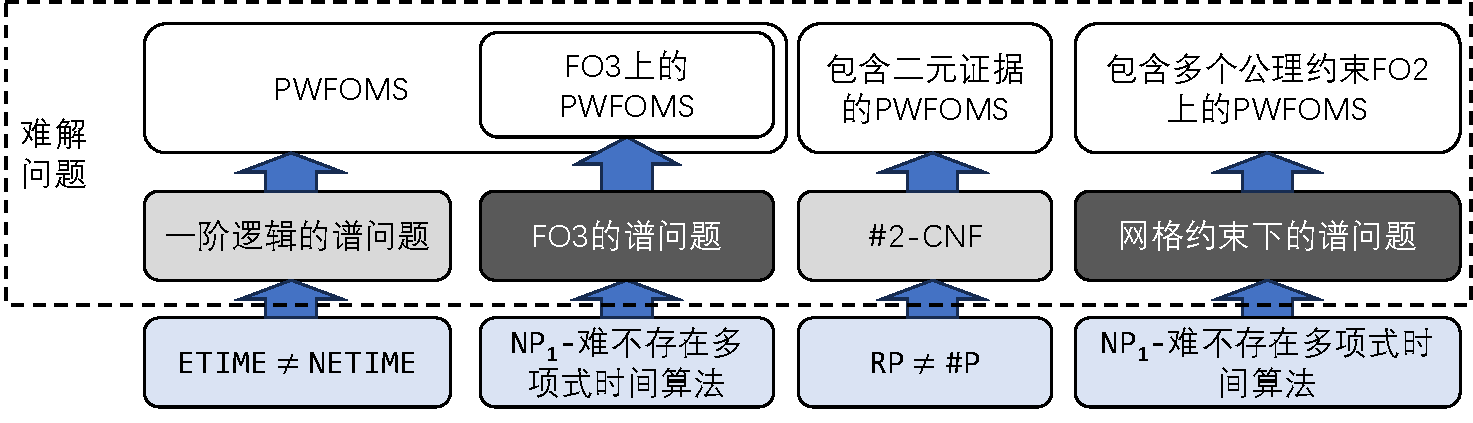
\includegraphics[width=\textwidth]{figs/hardness.pdf}
  \caption{一阶逻辑模型采样问题难解性的证明思路}
  \label{fig:hardness}
\end{figure}


\subsubsubsection{(1)全一阶逻辑上的模型采样问题难解性}

下面考虑PWFOMS问题的输入逻辑语句不包含二元证据的情况。
首先考虑全一阶逻辑上的模型采样问题,即所有(可包含等式关系)的一阶逻辑语句的模型采样问题。
对于该问题的难解性,可以通过对一阶逻辑谱问题的归约来证明。

\begin{problem}[一阶逻辑的谱问题]\label{prob:fo_spectrum}
  \ \\
  \textbf{给定:} 一个一阶逻辑语句$\sentence$\\
  \textbf{输入:} 一个正整数$n$\\
  \textbf{输出:} $\sentence$是否在大小为$n$的域上存在模型
\end{problem}

记一个一阶逻辑语句$\sentence$所有模型大小的集合为$spec(\sentence)$(又称作$\sentence$的谱),则一阶逻辑的谱问题即判断$n\in spec(\sentence)$。
对于任意的一阶逻辑谱问题$n \in spec(\sentence)$,构建一个\wfoms{}问题$(\sentence, n, \mathds{1}, \mathds{1})$,其中$\mathds{1}$是一个恒等于$1$的函数。
如果存在一个与$n$成多项式时间的算法\textsc{algo},可以解决该\wfoms{}问题,令$T$为\textsc{algo}在该\wfoms{}问题上的运行时间,则可以通过以下算法解决一阶逻辑的谱问题:在$(\sentence, n, \weight, \negweight)$上运行\textsc{algo},如果\textsc{algo}能够在$T$时间内输出一个模型,则输出“存在”;否则输出“不存在”。
显然上述算法的运行时间也是多项式的,所以可以得到以下结论。

\begin{proposition}\label{prop:pwfoms_spectrum}
  如果存在一个多项式时间算法,可以解决PWFOMS问题,那么也存在一个多项式时间算法,可以解决一阶逻辑的谱问题。
\end{proposition}

然而,已知除非$\mathsf{ETIME} = \mathsf{NETIME}$\footnote{
$\mathsf{ETIME} = \bigcup_{c>0} \mathsf{TIME}(2^{cn})$,$\mathsf{NETIME} = \bigcup_{c>0} \mathsf{NTIME}(2^{cn})$,即$\mathsf{ETIME}$和$\mathsf{NETIME}$分别是确定性图灵机和非确定性图灵机的指数时间复杂度类。},否则一定存在一个一阶逻辑语句$\sentence$,使得其谱问题不可在多项式时间内可解。
再由上述结论,可以得到全一阶逻辑上的模型采样问题的难解性。
\begin{theorem}
  除非$\mathsf{ETIME} = \mathsf{NETIME}$,否则PWFOMS问题不存在与$n$成多项式时间的算法。
\end{theorem}
% 实际上,一阶逻辑的谱问题等价于$\mathsf{NETIME}$,令$k$为$n$的二进制表示,则一个整数集合$S$是一个一阶逻辑语句$\sentence$的谱当且仅当$S$能够被非确定性图灵机在$2^{c\cdot|k|}$时间内判定。
% 因此,上述结论可以进一步推广到PWFOMS问题近似算法的难解性。

% 定义PWFOMS近似算法的近似比例为$\epsilon$,如果对于$\sentence$的任意模型$\mu$,其采样概率$P$满足$1 / (1+\epsilon)\pro[\mu\mid\sentence] \leq P \leq (1+\epsilon)\pro[\mu\mid\sentence]$。
% 假设PWFOMS问题存在一个与域大小$n$和$1/\epsilon$成多项式关系的近似算法,则可以通过类似上述的归约方法,证明一阶逻辑的谱问题同样存在一个与$1/\epsilon$成多项式关系的近似算法:给定一个一阶逻辑语句$\sentence$,可以构建一个\wfoms{}问题$(\sentence, n, \mathds{1}, \mathds{1})$;令$\epsilon=1/2$,在该\wfoms{}问题上运行近似算法,如果在多项式时间内输出一个模型,则输出“存在”;否则输出“不存在”。
% 由近似比的定义,可知若$n\in spec(\sentence)$,近似算法输出$\sentence$模型的概率(即输出“存在”的概率)大于等于$1 / (1+\epsilon) \sum_{\mu} \pro[\mu\mid\sentence] \geq 2/3$,若$n\notin spec(\sentence)$,输出“不存在”的概率也大于等于$2/3$。
% 因此通过上述归约,证明了若PWFOMS问题存在一个近似比为$1/2$的与$n$成多项式时间的近似算法,则一阶逻辑的谱问题存在一个误判率不超过$1/3$的多项式时间随机算法

% \begin{theorem}
%   若
%   除非$\mathsf{BPP} = \mathsf{NETIME}$,否则PWFOMS问题不存在近似比为$1/2$的多项式时间近似算法。
% \end{theorem}


\subsubsubsection{(2)\fothree{}上的模型采样问题难解性}

本项目进一步研究限定逻辑变量个数的情况下,PWFOMS问题的难解性。
由已知结论,\fotwo{}上的WFOMS问题是多项式时间可解的,那么该结论是否可以推广到\fothree{}?
% 该部分研究内容拟从两个方面展开:一是\emph{包含等式关系}的\fothree{}的模型采样问题,二是\emph{不包含等式关系}的\fothree{}的模型采样问题。
% 不包含等式关系的\fothree{}是\fothree{}的进一步细化,逻辑式中不包含形如$x=y$的等式关系。

该部分拟采用的技术路线仍为将PWFOMS问题归约到一阶逻辑的谱问题,进而证明PWFOMS问题的难解性,但该部分使用一元语言(Unary Language)的复杂类作为研究对象。
一元语言是一种特殊的只包含单一符号“$1$”的形式化语言,例如$\{1, 11, 111\}$,$\{1^k\mid k\text{是素数}\}$等,其又被称作计数语言(TALLY)。
对于一元语言的复杂类研究,相比于一般的形式化语言,有着更为特殊的性质,其最根本的区别在于使用的确定性图灵机和非确定性图灵机只能接受一元语言输入。
定义一元语言上的$\P$类为$\P_1$,为所有可以被确定性图灵机在多项式时间内判定的一元语言集合。同理,定义一元语言上的$\NP$类为$\NP_1$,为所有可以被非确定性图灵机在多项式时间内判定的一元语言集合。
定义两个一元语言上的问题$C_1$和$C_2$的多项式时间归约关系为:
\begin{definition}[多项式时间归约]
  给定两个一元语言上的问题$C_1$和$C_2$,令$f$为$C_1$的一个预言机,若存在一个可以执行$f$的确定性图灵机$T_{det}$,对于$C_2$的任意实例$x$(注意$x$是一元的),可以在$x$长度的多项式时间内判定$x\in C_2$,则称$C_2$可以多项式时间归约到$C_1$。
\end{definition}
\begin{definition}[$\NP_1$-难问题]
  一个一元语言上的问题$C$是$\NP_1$-难的,如果对于任意的一元语言上的问题$C'$,$C'$可以多项式时间归约到$C$。
\end{definition}

上述定义的$\NP_1$-难问题对应一般的$\NP$-难问题,可以理解为一元语言上的最难问题。
类似一般形式化语言的复杂类研究,通常认为$\NP_1$-难问题是不存在多项式时间算法的,即$\NP_1$-难问题不等于$\P_1$。
若一个问题$C$是$\NP_1$-难的,且$C\in\NP_1$,则称$C$是$\NP_1$-完全问题。
下面将给出证明PWFOMS问题是$\NP_1$-难的一个可行思路。

首先需要证明\fothree{}的谱问题是$\NP_1$-完全的。
谱问题显然是一个可以被非确定性图灵机在多项式时间内判定的问题,所以谱问题属于$\NP_1$。
\fothree{}谱问题的$\NP_1$-难证明主要分为两步:1)构造一个通用的$\NP_1$图灵机$U_1$,其可以在线性时间内判定一个$\NP_1$-完全问题的实例;2)构造一个\fothree{}逻辑语句$\sentence$模拟$U_1$的运行过程,证明$n\in spec(\sentence)$当且仅当$U_1$能够接受输入$n$。

\begin{lemma}\label{le:universal_np1}
  存在一个非确定性图灵机$U_1$,使得1)$U_1$运行时间是线性的;2)$U_1$定义了一个$\NP_1$-完全问题,即$\{1^k\mid 1^k\text{被}U_1\text{接受}\}$是$\NP_1$-完全的。
\end{lemma}

\begin{figure}[tb]
  \centering
  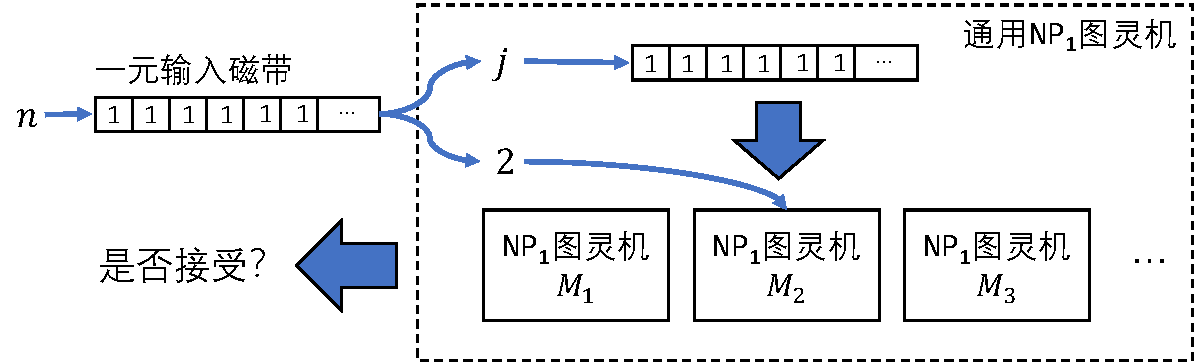
\includegraphics[width=.85\textwidth]{figs/NP1_TM.pdf}
  \caption{非确定性图灵机$U_1$的构造}
  \label{fig:np1_tm}
\end{figure}

上述引理的证明可以参照一般的$\NP$-完全问题存在性的证明方法,如\cref{fig:np1_tm}所示,采用配对函数的构造方法,将每个一元语言输入的图灵机$M$与其运行时间进行配对,从而构造一组$M_i$,使得$M_i$在输入$j$上的运行时间$\leq (i\cdot j^i+i)^2$。
给定一个一元输入$n$,$U_1$首先通过一个特定函数$e$计算出$i$和$j$,然后模拟$M_i$在输入$j$上的运行过程,最后输出$M_i$的判定结果。
通过对$e$的设计,可以保证$U_1$的运行时间是线性的。
同时,对于任意$\NP_1$问题输入$j$,存在一个非确定性图灵机$M$,使得$M$可以判定$j$。
因此,可以通过先计算$n = e(i, j)$,再调用$U_1$来判定$n$,可以容易的证明$n$被$U_1$接受当且仅当$M$接受$j$。

当有了\cref{le:universal_np1}的结论后,可以通过构造一个\fothree{}的逻辑语句$\sentence$来证明PWFOMS问题的$\NP_1$-难性。
具体来说,有如下的引理。
\begin{lemma}\label{le:fo3_turing}
  给定一个以一元语言输入的非确定性图灵机$M$,如果$M$可在线性时间$O(n)$内判定输入$1^n$,则存在一个包含等式关系的\fothree{}逻辑语句$\sentence$,使得$n\in spec(\sentence)$当且仅当$M$接受$1^n$。
\end{lemma}

上述引理的证明可由Trakhtenbrot的证明方法推广而来,Trakhtenbrot证明了对于任意确定性图灵机$M$,存在一个一阶逻辑语句$\sentence$,使得$\sentence$是可满足的当且仅当$M$接受空输入。
在Trakhtenbrot的证明中,$\sentence$是由$\{<, Min, T_0, T_1, H, (Sq)q\in States(T)\}$构成的一阶逻辑语句,其中$<$是一个全序关系,$Min(x)$表示$x$是全序关系的最小元素,$T_0(t, p)$(或$T_1(t, p)$)表示在时间$t$时,磁带的位置$p$上为$0$(或$1$),$H(t, p)$表示在时间$t$时,磁头在位置$p$上,$Sq(t)$表示在时间$t$时,机器处于状态$q$。
\cref{le:fo3_turing}的证明需要对Trakhtenbrot的证明进行适当的修改,主要包括:1)将确定性图灵机$M$替换成非确定性图灵机$M$,2)图灵机的输入从空输入变为一元输入$1^n$,3)图灵机有$k$条磁带,4)图灵机的运行时间限制为$O(n)$,5)$\sentence$属于\fothree{}。
以上5点修改理论上都是可行的,具体的构造细节此处不再赘述。
由\cref{le:universal_np1}和\cref{le:fo3_turing},以及一阶逻辑的谱问题到PWFOMS问题的归约(\cref{prop:pwfoms_spectrum}),可以得到以下结论。
\begin{theorem}
  \fothree{}的谱问题是$\NP_1$-完全的。
\end{theorem}
\begin{theorem}\label{thm:fo3_hard}
  \fothree{}的PWFOMS问题是$\NP_1$-难的。
\end{theorem}

% 类似的,由一阶逻辑谱问题的随机算法到PWFOMS近似算法的归约,可以得到以下推论。
% \begin{corollary}\label{cor:fo3_approx}
%   若$\NP_1$-完全问题不存在误判率不超过$1/3$的多项式时间近似算法,则包含等式关系的\fothree{}上,PWFOMS问题不存在近似比为$1/2$的多项式时间近似算法。
% \end{corollary}

% 由\cref{cor:fo3_approx},可以将PWFOMS的难解性进一步推广至不包含等式关系的\fothree{}上。
% 首先,对于任意包含等式关系的\fothree{}语句$\sentence$,可以将其中所有$x=y$的原子式替换成$E(x,y)$,其中$E$是一个新的二元谓词,并将$\forall x: E(x,x)$加入到$\sentence$中,从而得到一个不包含等式关系的\fothree{}语句$\sentence'$。
% 易知,$\sentence$上的PWFOMS问题等价于$\sentence'\land |E| = n$上的PWFOMS问题,其中$|E| = n$表示基数约束,即模型中$E$为真的元组个数为$n$。
% 可以进一步去除基数约束,将谓词$E$的权重$w(E)$设置成一个足够小的值,从而使得$|E| > n$的所有模型的采样概率趋近于$0$,即采样$|E| = n$(由于$\forall x: E(x,x)$的约束)模型的概率趋近于$1$。
% 利用上述方法,可以容易的将包含等式关系的\fothree{}的模型近似采样问题归约到不包含等式关系的\fothree{}的模型(近似)采样问题,则可以得到以下结论。

% \begin{theorem}
%   若$\NP_1$-完全问题不存在误判率不超过$1/3$的多项式时间近似算法,则不包含等式关系的\fothree{}上,PWFOMS问题不存在(近似比为$1/2$)的多项式时间(近似)算法。
% \end{theorem}

\subsubsubsection{(3)包含二元证据的模型采样问题难解性}

对于包含二元证据的WFOMS问题难解性分析,考虑$\#2$-CNF问题:计算一个$2$-CNF语句的所有模型个数。
关于$\#2$-CNF问题,已有的工作证明除非$\R\P=\#\P$,否则其不存在多项式时间的近似算法,所以可以直接推论其对应的采样问题也不存在多项式时间的算法。
\begin{theorem}
  除非$\R\P=\#\P$,否则在输入逻辑式可满足的情况下,$2$-CNF的采样问题不存在多项式时间的算法。
\end{theorem}
% 对于任意的2-CNF采样问题,可以将其转化成一个包含二元证据的WFOMS问题:
\begin{lemma}\label{lem:2cnf_to_fo2}
    任意的2-CNF语句可以表示成包含二元证据的$\mathbf{FO}^2$语句:
    \begin{align*}
        P(X)\lor P(Y)\lor \neg C_1(X,Y)\\
        P(X)\lor \neg P(Y)\lor \ng C_2(X,Y)\\
        \neg P(X)\lor \neg P(Y)\lor \neg C_3(X,Y)
    \end{align*}
    其中,每个$\mathbf{FO}^2$语句都是由全称量词限制。
\end{lemma}
可以通过设置不同的$C_i$的取值,将2-CNF语句转化成上述逻辑语句在二元证据下的实例化。
例如,在二元证据$C_1(a,b)$的情况下,上述逻辑语句实例化为$p(a)\lor p(b)$。
一个否定的二元证据$\neg C_i(a,b)$则表示其对应的子句不在逻辑语句中,例如$\neg C_2(a,b)$表示$p(a)\lor \neg p(b)$不在逻辑语句中。
以$(p(a)\lor p(b)) \land (p(a)\lor \neg p(c)) \land (\neg p(c)\lor \neg p(d))$为例,其对应的二元证据为$C_1(a,b)\land \neg C_1(a,a)\land \dots \land \neg C_1(d,d)\land C_2(a,c)\land \neg C_2(a,a)\land \dots \land \neg C_2(d,d)\land C_3(c,d)\land \neg C_3(a,a)\land \dots \land \neg C_3(d,d)$。

通过上述引理和2-CNF采样问题的不可高效求解,可以证明除非$\RP=\#\P$,包含二元证据的PWFOMS问题不存在多项式时间算法。
\begin{theorem}
    假设PWFOMS问题允许输入逻辑语句中包含二元证据,那么除非$\R\P=\#\P$,否则不存在与二元证据个数呈多项式时间的模型采样算法。
\end{theorem}
注意\cref{lem:2cnf_to_fo2}中的逻辑语句只包含两个逻辑变量,即为\fotwo{}语句,所以上述结论可进一步推论。
\begin{corollary}
  除非$\R\P=\#\P$,否则\fotwo{}上,不存在与二元证据个数呈多项式时间的模型采样算法。
\end{corollary}

\subsubsubsection{(4)包含多个公理约束的模型采样问题难解性}

最后,对于包含多个公理约束\fotwo{}上的模型采样问题,本项目拟通过\emph{网格约束}的构造,将其归约到一元语言上的$\NP_1$-完全问题,从而证明其难解性。
网格约束$grid(H, V)$也是一种公理约束,其要求:
\begin{itemize}
  \item 二元谓词$H$和$V$构成的图是一个方形网格图,
  \item 对于任意的$x,y$,$H(x,y)$表示$x$和$y$在同一行,且$y$是$x$的直接后继,
  \item 对于任意的$x,y$,$V(x,y)$表示$x$和$y$在同一列,且$y$是$x$的直接后继。
\end{itemize}
类似上述证明\fothree{}的PWFOMS问题难解性,可以通过构造一个包含网格约束的\fotwo{}的逻辑语句$\sentence$,证明其谱问题是$\NP_1$-完全的。
\begin{theorem}\label{thm:grid_hard}
  包含网格约束的\fotwo{}上的谱问题是$\NP_1$-完全的。
\end{theorem}

上述定理的证明可以采用与\fothree{}的PWFOMS问题难解性类似的方法:构造与通用$\NP_1$非确定性图灵机$U_1$的逻辑语句$\sentence$,证明$n\in spec(\sentence)$当且仅当$U_1$接受$1^n$。
具体的构造方法与证明平铺问题是不可判定的证明方法类似,网格的第$i$行表示$U_1$在第$i$步的状态,$U_1$的状态转移通过约束$H$和$V$来表示,从而模拟$U_1$的运行过程。

基于包含网格约束的\fotwo{}上谱问题的难解性,可以证明多个公理约束下的模型采样问题的难解性。
主要思路是利用包含多个公理约束的\fotwo{}逻辑语句,模拟网格约束,从而将包含网格约束的\fotwo{}上的谱问题归约到多个公理约束下的PWFOMS问题。
下面以线性序公理约束$LO$为例,给出一个具体的模拟方法。


\begin{figure}[tb]
  \centering
  \begin{subfigure}[t]{0.4\textwidth}
      \centerline{
      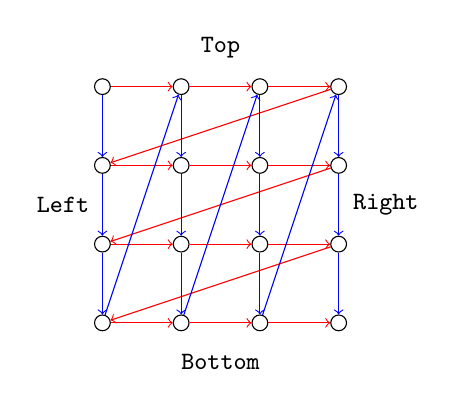
\begin{tikzpicture}
        \tikzstyle{roundnode}=[circle, draw, inner sep=0pt, minimum size=2mm]
        \foreach \i in {0,1,2,3}
            \foreach \j in {0,1,2,3}
                \node[roundnode] (a\i\j) at (\i,\j) {};
        \foreach \i in {0,1,2} {
            \foreach \j in {0,1,2,3}
                \pgfmathtruncatemacro{\k}{\i+1}
                \path[->,red] (a\i\j) edge (a\k\j);
            \pgfmathtruncatemacro{\k}{\i+1}
            \path[->,red] (a3\k) edge (a0\i);
        }
        \foreach \j in {0,1,2} {
            \foreach \i in {0,1,2,3}
                \pgfmathtruncatemacro{\k}{\j+1}
                \path[->,blue] (a\i\k) edge (a\i\j);
            \pgfmathtruncatemacro{\k}{\j+1}
            \path[->,blue] (a\j0) edge (a\k3);
        }
        \node[] (Top) at (1.5,3.5) {\small \texttt{Top}} ;
        \node[] (Bottom) at (1.5,-0.5) {\small \texttt{Bottom}} ;
        \node[] (Left) at (-0.5,1.5) {\small \texttt{Left}};
        \node[] (Right) at (3.6,1.5) {\small \texttt{Right}};
      \end{tikzpicture}
      }
    \caption{基于线性序$L_1$(红色箭头)和$L_2$(蓝色箭头)的网格约束构建}\label{fig:L1L2}
  \end{subfigure}
  \hspace{1cm}
  \begin{subfigure}[t]{0.4\textwidth}
      \centerline{
      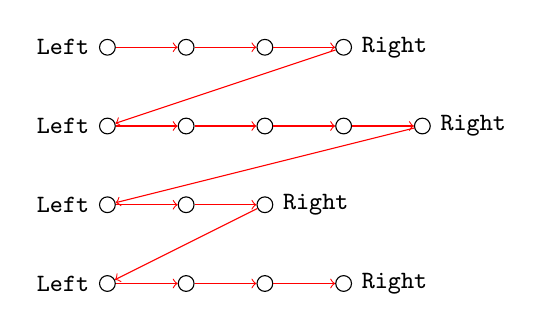
\begin{tikzpicture}
        \tikzstyle{roundnode}=[circle, draw, inner sep=0pt, minimum size=2mm]
        \tikzstyle{roundnodeleft}=[circle, draw, inner sep=0pt, minimum size=2mm, label=left:{\small \texttt{Left}}]
        \tikzstyle{roundnoderight}=[circle, draw, inner sep=0pt, minimum size=2mm, label=right:{\small \texttt{Right}}]
        \foreach \j in {0,3} {
            \node[roundnodeleft] (a0\j) at (0,\j) {};
            \foreach \i in {1,2} \node[roundnode] (a\i\j) at (\i,\j) {};
            \node[roundnoderight] (a3\j) at (3,\j) {};
            \foreach \i in {0,1,2}
                \pgfmathtruncatemacro{\k}{\i+1}
                \path[->,red] (a\i\j) edge (a\k\j);
        }
        \node[roundnodeleft] (a02) at (0,2) {};
        \node[roundnoderight] (a42) at (4,2) {};
        \foreach \i in {1,2,3} \node[roundnode] (a\i2) at (\i,2) {};
        \foreach \i in {0,1,2,3}
            \pgfmathtruncatemacro{\k}{\i+1}
            \path[->,red] (a\i2) edge (a\k2);
        \node[roundnodeleft] (a01) at (0,1) {};
        \node[roundnode] (a11) at (1,1) {};
        \node[roundnoderight] (a21) at (2,1) {};
        \path[->,red] (a01) edge (a11);
        \path[->,red] (a11) edge (a21);
        \path[->,red] (a33) edge (a02);
        \path[->,red] (a42) edge (a01);
        \path[->,red] (a21) edge (a00);
      \end{tikzpicture}
      }
    \caption{\Cref{eq:LeftRight1}约束下$L_1$的形状}\label{fig:L1-1}
  \end{subfigure}
  \caption{模拟网格约束的线性序}\label{fig:L1L2-1}
\end{figure}

给定一个线性序,可以定义其首元素关系$First$和末元素关系$Last$,以及后继关系$S$。
下面将使用两个线性序$LO(R_1)$和$LO(R_2)$来模拟网格约束,其中$R_1$和$R_2$是两个二元关系,如\cref{fig:L1L2}所示。
为简洁起见,使用$L_1$和$L_2$来表示$LO(R_1)$和$LO(R_2)$,并且假设域大小$n \ge 2$。
令$S_1$和$S_2$分别表示$L_1$和$L_2$的后继关系,$First_1$和$First_2$表示$L_1$和$L_2$的首元素关系,$Last_1$和$Last_2$表示$L_1$和$L_2$的末元素关系。
首先,约束$L_1$的形状,将$L_1$的元素分为左侧和右侧两部分,使用$Left$和$Right$来表示。
\begin{equation}\label{eq:LeftRight1}
  \begin{aligned}
    & |Left| = |Right| = n \\
    \land & \forall x ((First_1(x) \to Left(x)) \land (Last_1(x) \to Right(x))) \\
    \land & \forall x (\lnot Left(x) \lor \lnot Right(x))\\
    \land & \forall x \forall y \left( S_1(x,y) \to (Right(x) \leftrightarrow Left(y)) \right).
  \end{aligned}
\end{equation}
在上式的约束下,$L_1$的形状如\cref{fig:L1-1}所示:$L_1$被分为$n$行,且每行至少有两个元素。
然后,约束模拟网格的第一行$Top$和最后一行$Bottom$,并约束$Top$和$Bottom$的长度为$n$。
\begin{equation}\label{eq:TopBottom}
  \begin{aligned}
    \forall x &\forall y (S_1(x,y) \land \lnot Right(x) \to (Top(x) \leftrightarrow Top(y)) \land (Bottom(x) \leftrightarrow Bottom(y))) \\
    \land & \forall x (First_1(x) \leftrightarrow Left(x) \land Top(x)) \\
    \land & \forall x (Last_1(x) \leftrightarrow Right(x) \land Bottom(x)) \\
    \land & |Top| = |Bottom| = n.
  \end{aligned}
\end{equation}
接下来,约束$L_2$的形状,$L_1$和$L_2$共享相同的首元素和末元素。
\begin{equation}\label{eq:L2-1}
  \forall x ((First_1(x) \leftrightarrow First_2(x)) \land (Last_1(x) \leftrightarrow Last_2(x))).
\end{equation}
最后,通过后继关系$S_1$和$S_2$来模拟网格的列。
\begin{equation}\label{eq:L2-2}
  \begin{aligned}
    & \forall x \forall y (S_1(x,y) \land \lnot Right(x) \to L_2(x,y)) \\
    \land & \forall x \forall y (S_2(x,y) \land \lnot Bottom(x) \to L_1(x,y)) \\
    \land & \forall x \forall y (\lnot S_1(x,y) \lor \lnot S_2(x,y)).
  \end{aligned}
\end{equation}
可以证明,基于上述约束,$L_1$和$L_2$的形状如\cref{fig:L1L2}所示,即模拟了一个网格的形状,网格中$H$和$V$的关系可以下式定义:
\begin{equation}
  \begin{aligned}
    & \forall x \forall y (H(x,y) \leftrightarrow S_1(x,y) \land \lnot Right(x)) \\
    \land & \forall x \forall y (V(x,y) \leftrightarrow S_2(x,y) \land \lnot Bottom(x)).
  \end{aligned}
  \label{eq:HV}
\end{equation}
所以,可以得到以下引理。

\begin{lemma}\label{lemma:grid_2lo}
  令$\sentence$为一个\fotwo{}逻辑语句,$\sentence'$为$\sentence$和\cref{eq:LeftRight1,eq:TopBottom,eq:L2-1,eq:L2-2,eq:HV}的合取,则$n\in spec(\sentence\land grid(H,V))$当且仅当$n\in spec(\sentence')$。
\end{lemma}

由上述引理和\cref{thm:grid_hard},可证包含两个线性序公理约束的\fotwo{}上的谱问题是$\NP_1$-完全的,从而证明其对应的PWFOMS问题的难解性。
\begin{theorem}
  包含两个线性序公理约束的\fotwo{}上的PWFOMS问题是$\NP_1$-难的。
\end{theorem}

\subsubsection{3.1.1 一阶逻辑模型采样问题的近似算法设计}

针对这一研究内容,拟采用的技术路线如下:对于包含二元证据的\wfoms{}问题,基于对$\mathbf{FO}^2$上采样算法的分析,利用\wfoms{}问题中一元类型和二元表的特点,设计分块吉布斯采样算法,实现高效的近似采样;
对于FO3上的WFOMS问题,研究当逻辑句中只包含二元谓词和全称量词的情况,利用二元表采样的独立性,同样基于分块吉布斯采样,设计并行化的模型近似采样算法;
对于一般的全一阶逻辑公式上的\wfoms{}问题,设计先采样谓词基数向量,再采样模型的近似采样算法,并通过对基数向量空间的分块划分,进一步提高采样算法的效率。

\subsubsubsection{(1)\fothree{}上的并行近似采样算法}

针对只包含一元、二元谓词和全称量词的\fothree{}语句,本项目拟采用Gibbs采样方法设计近似采样算法。
吉布斯采样(Gibbs Sampling)是一种马尔科夫链蒙特卡洛方法,多用于高维概率分布的采样,在概率图模型、概率推理、统计学习等领域有着广泛的应用。

对于给定的WFOMS问题$(\sentence, \domain,\weight, \negweight)$,可以首先将$\sentence$在$\domain$上进行实例化,从而得到一个命题逻辑式$\Pi$, 其中不包含任何逻辑变量和量词。
实例化后的命题逻辑式$\Pi$可以看作定义了一个马尔科夫网络,其中每个布尔变量对应一个随机变量,每个子句对应一个团,$\Pi$及$\weight, \negweight$定义了团的势函数。
由此,一个WFOMS问题即可转化成马尔科夫网络上的采样问题。

基于Gibbs采样,首先随机生成马尔科夫网络中各个随机变量的真值
\begin{equation*}
    \bar{\vecx}^{(0)} = (\bar{x}_1^{(0)}, \bar{x}_2^{(0)}, \dots, \bar{x}_n^{(0)})
\end{equation*}
然后进行$T$步的迭代,对于每一步$t$,对变量的真值进行如下更新:对于$i=1, 2, \dots, n$,依以下概率
\begin{equation}
    \pro[X_i\mid \bar{x}_1^t, \dots,\bar{x}_{i-1}^t, x_{i+1}^{t-1},\dots, x_n^{t-1}]
    \label{eq:gibbs}
\end{equation}
更新$\bar{x}^{t-1}$为$\bar{x}^t$。
为了描述简洁,令$\bar{\vecx}_{-i}^{(t)} = (\bar{x}_1^{(t)}, \dots, \bar{x}_{i-1}^{(t)}, \bar{x}_{i+1}^{(t-1)}, \dots, \bar{x}_n^{(t-1)})$,并记Gibbs采样中,每次迭代的概率\Cref{eq:gibbs}为$\pro[X_i\mid \bar{\vecx}_{-i}^{(t)}]$。
当$X_i$更新完成,令$t+1$,当所有$T$步更新完成,最后的$\bar{\vecx}^T$即为采样出的真值,也即$\Pi$($\sentence$)的一个模型。
上述对于真值的更新过程可以看作是一个马尔科夫链,根据其非周期性和遍历性,可以证明上述更新过程一定收敛于概率分布$\pro[\vecx\mid \Pi;\weight, \negweight] = \pro[\mu\mid \Pi;\domain, \weight, \negweight]$,其中$\mu$是$\vecx$对应的$\sentence$的模型。
上述的Gibbs采样适用于一般的WFOMS问题,但由于Gibbs采样通常需要很长的迭代步数才能收敛,从而采样算法的效率十分低下。
因此,本项目考虑\fothree{}上WFOMS问题蕴含的结构特点,拟采用更加高效的分块Gibbs采样算法设计近似采样算法。

\emph{分块Gibbs}采样算法的主要思想是将随机变量进行分组,在进行迭代时,每次针对每一组中的所有随机变量进行统一迭代。
当分组合理时,分块Gibbs可以大幅提升Gibbs迭代的收敛速度。
然而当随机变量的分组不合理(例如某组中随机变量的边缘分布的树宽(treewidth)较大)时,每次Gibbs迭代只能通过暴力的枚举采样得到整组变量的更新值,从而导致分块Gibbs的效果可能不如Gibbs采样。
所以,分块Gibbs的分组方法对于算法的效率有着至关重要的影响。

通过分析$\mathbf{FO}^2$的精确采样算法,可以发现若一阶逻辑语句中只包含一元、二元谓词,采样问题可以分解成对于常量的一元类型(注意此时无需考虑常量格类型中包含的块类型)采样,以及对常量对的二元表采样。
若一阶逻辑只包含全称量词,不含任何存在量词,则逻辑式可以写成
\begin{equation*}
    \sentence = \forall x_1\forall x_2\dots\forall x_k: \fotwoformula(x_1,\dots,x_k)
\end{equation*}
其中$\fotwoformula(x_1,\dots,x_k)$是一个无量词逻辑式。
下面以$k=3$,即\fothree{}为例,此时$\sentence$可以写成$\forall x\forall y\forall z: \fotwoformula(x,y,z)$。
将其在常量域$\domain$上gounding后,可以得到$\sentence = \bigwedge_{i,j,k \in[n]}\fotwoformula(e_i, e_j, e_k)$。
当常量的一元类型固定时,将其对应的一元原子式真值带入上式中,可以发现对于任意的$\{i, j\}\cap \{i', j'\}=\emptyset$,$\fotwoformula(e_i, e_j, e_{i'})$不可能同时包含$(e_{i'}, e_{j'})$的二元表中的任意原子式和$(e_{i'}, e_{j'})$的二元表中的任意原子式,因此,$(e_i, e_j)$的二元表采样独立于$(e_{i'}, e_{j'})$的二元表采样。

可以采用图着色方法来发现在一元类型固定时,所有独立的二元表。
假设常量域大小为$n$,首先构造一个大小为$n$的完全图;然后,利用图着色方法寻找图中最小的边着色,因为此时考虑的是完全图,所以这一步显然是可高效求解的;最后,根据边的颜色,所有具有相同颜色的边对应的常量二元组的二元表是独立的。
如\cref{fig:graph_coloring}所示,对于$n=6$的情况,得到了五种颜色的边,即有五种相互独立的二元表。
容易证明,若$n$为偶数,共需要$n-1$种颜色进行着色,若$n$为奇数,则需要$n$种颜色。

\begin{figure}[!htb]
   \centering
   \begin{minipage}[t]{.3\textwidth}
    \centering
    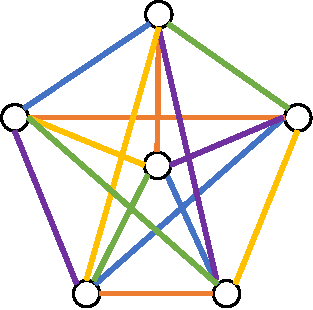
\includegraphics[width=\linewidth]{figs/gpu_gibbs.pdf}
    \caption{图着色示例}
    \label{fig:graph_coloring}
   \end{minipage}
   \hspace{1cm}
   \begin{minipage}[t]{.6\textwidth}
    \centering
    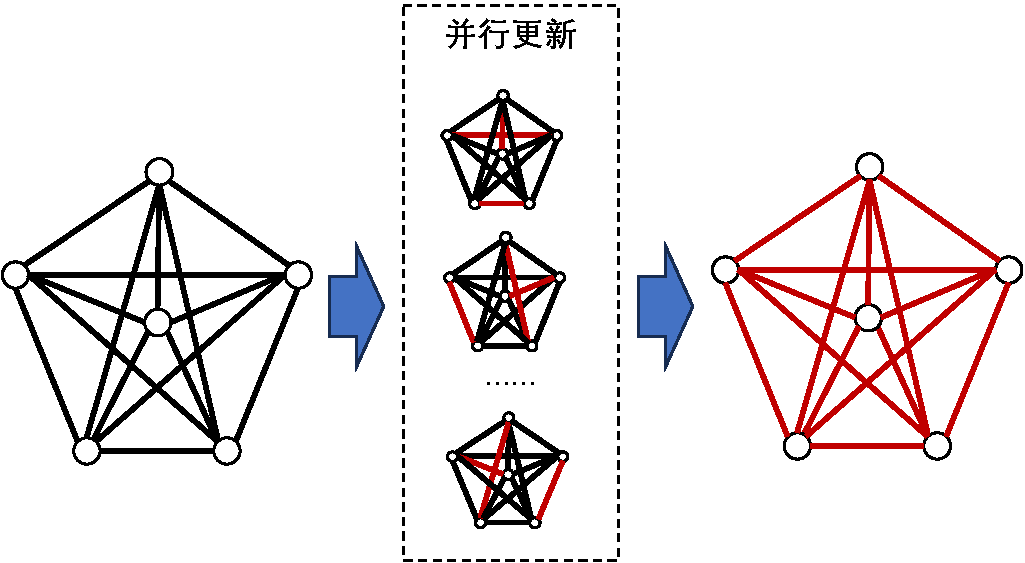
\includegraphics[width=\linewidth]{figs/FO3_sampling.pdf}
    \caption{并行更新$\bar{\vecx}_{\mathcal{C}_q}$示例}
    \label{fig:gpu_gibbs}
   \end{minipage}
\end{figure}

基于分块Gibbs和上一部分对于二元证据的近似采样算法设计,可以设计针对\fothree{}的近似采样算法。
将WFOMS对应的马尔科夫网络中的随机变量分割成:
\begin{itemize}
  \item 对于每个常量$e_i\in\domain$,令其一元类型中包含的随机变量为一组,记为$[\mathbf{X}]_{e_i}$,即所有只和$e_i$有关的随机变量,
  \item 图着色中每种颜色$\mathcal{C}_q$对应的二元表中包含的随机变量为一组,记为$\mathbf{X}_{\mathcal{C}_q}$。
\end{itemize}
拟采用的分块Gibbs算法的第$t$步迭代过程如下:
\begin{itemize}
    \item 对于每个常量$e_i\in\domain$,以概率$\pro\left[[X]_{e_i}\mid [\bar{\vecx}^{(t)}]_{\mathbf{e}_{-i}}, \bar{\vecx}_{\mathcal{C}_1}^{(t)},\dots,\bar{\vecx}_{\mathcal{C}_Q}^{(t)}\right]$更新$[\bar{\vecx}^{(t-1)}]_{e_i}$为$[\bar{\vecx}^{(t)}]_{e_i}$;
    \item 对于每个$q\in[Q]$,以概率
    \begin{equation*}
        \pro\left[\mathbf{X}_{\mathcal{C}_q}\mid [\bar{\vecx}^{(t)}]_{e_1},\dots,[\bar{\vecx}^{(t)}]_{e_n},\bar{\vecx}^{t-1}_{\mathcal{C}_1},\dots, \bar{\vecx}^{t-1}_{\mathcal{C}_{q-1}}, \bar{\vecx}^{t-1}_{\mathcal{C}_{q+1}},\dots, \bar{\vecx}^{t-1}_{\mathcal{C}_{Q}}\right]
    \end{equation*}
    更新$\bar{\vecx}_{\mathcal{C}_q}^{(t-1)}$为$\bar{\vecx}_{\mathcal{C}_q}^{(t)}$。
\end{itemize}
上述过程中,对于$\bar{\vecx}_{\mathcal{C}_q}$的更新可以再次分块使用Gibbs采样算法,把$\bar{\vecx}_{\mathcal{C}_q}$中每个二元表中的随机变量分为一组,进行迭代更新。
可以看到,上述算法的第二步$\bar{\vecx}_{\mathcal{C}_q}^{(t)}$的更新中,对于任意$q_1\neq q_2$,$\bar{\vecx}_{\mathcal{C}_{q_1}}^{(t)}$和$\bar{\vecx}_{\mathcal{C}_{q_2}}^{(t)}$的更新是独立的,因此该步的更新可以对$q$并行进行,从而可以设计并行Gibbs采样算法。
如\cref{fig:gpu_gibbs}所示,给出了$n=6$的情况下的更新$\bar{\vecx}_{\mathcal{C}_q}$一步的示例。
上述并行Gibbs采样算法可进一步优化,通过GPU并行计算,提高算法的效率。

\subsubsubsection{(3)全一阶逻辑上的近似采样算法}

针对一般的全一阶逻辑语句上的\wfoms{}问题,本项目拟设计一种基于基数分块的近似采样算法,且该算法具有一定的近似保证。

考虑一个\wfoms{}问题$(\sentence, \domain, \weight, \negweight)$。
记$\sentence$的模型$\mu$上谓词$P$的基数为$N(P, \mu)$,即$\mu$中满足$P$的实例个数。
假设$\sentence$中包含$m$个谓词$P_1, \dots, P_m$,令$\cardinality(\sentence, \mu) = (N(P_1, \mu), \dots, N(P_m, \mu))$。
给定一个整数向量$\veck=(k_1,\dots, k_m)\in\nat^m$,定义
\begin{equation*}
  \symfomc_{\sentence,\domain}(\veck) := \sum_{\mu\in\fomodels{\sentence}{\domain}} \indicator[\cardinality(\sentence, \mu) = \veck]
\end{equation*}
则该\wfoms{}问题中的采样概率可以写成
\begin{equation}
    \pro[\mu\mid \sentence, \domain, \weight, \negweight] = \frac{\symfomc_{\sentence,\domain}(\cardinality(\sentence, \mu))\cdot \typeweight{\mu}}{\symwfomc(\sentence, \domain, \weight, \negweight)}\cdot \frac{1}{\symfomc_{\sentence,\domain}(\cardinality(\sentence, \mu))}
\end{equation}
其中$\mathcal{K}$是所有可能的基数向量集合。
不难看出,上式求和号内的两个分式都是一个概率分布,第一个分式定义了基数向量$\veck$的分布,第二个分式定义了给定$\veck$模型的均匀分布。
因此,可以将\wfoms{}问题分解为两个部分:基数采样问题和基数向量$\veck$给定的均匀采样问题。
下面将分别介绍这两个问题的近似算法。
相比于直接从$\fomodels{\sentence}{\domain}$中采样,分步采样的好处在于:1)基数约束限制了采样空间,使得采样可能更加高效;2)均匀采样无需考虑模型权重,简化了算法设计。

首先考虑给定基数向量$\veck$的均匀采样问题。
该问题可以通过将$\sentence$实例化为命题逻辑式$\Pi$,然后使用命题逻辑上的模型近似采样算法进行采样。
本项目拟采用目前最好的命题逻辑模型采样算法Unigen,该算法的主要优势是可以保证采样结果近似服从均匀分布,即算法输出$\structure$的概率$\pro[\structure]$满足$\frac{1}{(1+\epsilon)\symfomc_{\sentence,\domain}(\veck)} \le \pro[\structure] \le \frac{1+\epsilon}{\symfomc_{\sentence,\domain}(\veck)}$。\footnote{Unigen算法依赖于SAT求解器,因此其时间复杂度没有保证,这也符合项目内容二预期的全一阶逻辑上\wfoms{}问题的难解性。}
Unigen算法的主要思路是将模型的采样空间分解为足够小的均匀的多个子空间,再通过调用SAT求解器遍历子空间内的所有模型。
在拟采用的分步采样算法中,由于基数约束的限制,采样空间进一步缩小,因此可以期望Unigen算法在该问题上有更好的效果。

下面考虑基数采样问题。
最直接的方法是直接枚举所有可能的基数向量,在根据每个基数向量的权重$\symfomc_{\sentence,\domain}(\veck)\cdot \typeweight{\veck}$进行采样。
然而,由于基数向量的个数与谓词个数成指数关系,直接枚举所有基数向量并非可行。
因此,本项目拟设计一个基于基数分块的近似采样算法。
具体来说,将基数向量空间$\mathcal{K}$分割成不相交的小矩形框,对于每个框和其中的一组整数点$\mathcal{C} = \{\mathbf{k}^{(1)}, \dots, \mathbf{k}^{(t)}\}$,计算
\begin{equation*}
  \symfomc_{\sentence,\domain}(\mathcal{C}) = \symfomc_{\sentence,\domain}(\mathbf{k}^{(1)}) + \dots + \symfomc_{\sentence,\domain}(\mathbf{k}^{(t)})
\end{equation*}
以及矩形框内模型权重的最小值和最大值
\begin{equation*}
  lb = \min_{j\in[t]}\prod_{i=1}^m \weight(P_i)^{k^{(j)}_i}\cdot \negweight(P_i)^{n^{arity(P_i)}-k^{(j)}_i}, 
  ub = \max_{j\in[t]} \prod_{i=1}^m \weight(P_i)^{k^{(j)}_i}\cdot \negweight(P_i)^{n^{arity(P_i)}-k^{(j)}_i},
\end{equation*}
其中$arity(P_i)$是谓词$P_i$的元数。
则矩形框$\mathcal{C}$内基数向量的权重之和可以由$\symfomc\linebreak_{\sentence,\domain}(\mathcal{C}) \cdot lb$和$\symfomc_{\sentence,\domain}(\mathcal{C}) \cdot ub$进行近似,从而基数向量的采样问题可以转化为先近似采样矩形框,再在矩形框内均匀采样的问题。
矩形框的分块策略可以由权重之和的上下界比值进行启发式选择,对于上下界较大(即权重估计不准)的矩形框,可以进一步分块,从而提高采样效率。
$\symfomc_{\sentence,\domain}(\mathcal{C})$的计算同样可以通过将其归约为命题逻辑模型计数问题进行求解,若采用具有理论保证的模型计数算法,如ApproxMC,则也可以保证采样结果的近似正确性。

最后,在上述基于基数分块的近似采样算法中,可以进一步通过提前计算基数向量的取值空间$\mathcal{K}$,即\wfoms{}问题对应的关系边际多面体(Relation Marginal Polytope),提高采样效率。
如\cref{fig:approxwfomc_split}所示,蓝色区域为基数向量的取值空间,若已知该区域,则在分块时可忽略不可能的基数向量(区域$3$和$4$),从而减少分块的矩形框数量。


\begin{figure}[tbp]
  \centering
  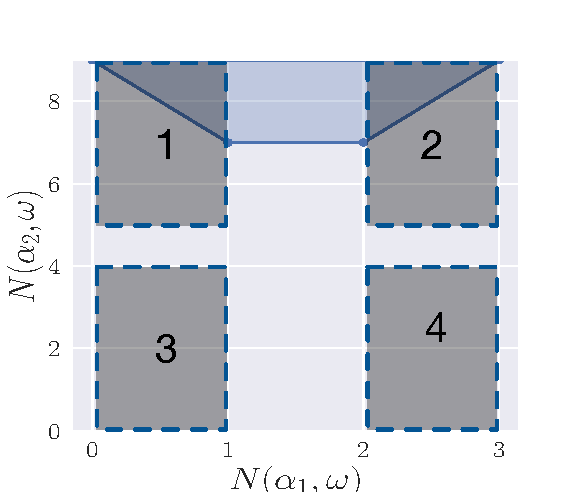
\includegraphics[width=.37\textwidth]{figs/approxwfomc_split.pdf}
  \caption{基于关系边际多面体的基数分块示例}
  \label{fig:approxwfomc_split}
\end{figure}


\subsubsubsection{(3)包含二元证据的近似采样算法}

对于包含二元证据的WFOMS问题,本部分研究拟同样基于分块吉布斯采样方法对其设计近似采样算法。

对于包含二元证据的WFOMS问题,通过深入分析不含二元证据$\mathbf{FO}^2$上的精确采样算法,可以发现算法的主要框架可以分成两个部分(由\cref{eq:sampling_cell_type}):1)采样域中每个常量的格类型;2)在格类型的条件下,采样所有常量二元组的二元表。
其中第二步当格类型固定的情况下,对于二元表的采样是可以高效进行的(时间复杂度是$n$的多项式)。
通过进一步分析,可知:即使在包含二元证据的情况下,二元表的采样也可在多项式时间内完成。
因此,本项目拟采用下述方法对于随机变量进行分组:
\begin{itemize}
    \item 对于每个常量$e_i\in\domain$,令其格类型中包含的随机变量为一组,记为$[\mathbf{X}]_{e_i}$,即所有只和$e_i$有关的随机变量,
    \item 其他所有二元表中对应的随机变量(不包含给定的二元证据)为另外一组,记为$\mathbf{X}_{B}$。
\end{itemize}
拟采用的分块Gibbs算法如下:
\begin{itemize}
    \item 随机初始化每组随机变量$[\bar{\vecx}^{(0)}]_{e_i}$和$\bar{\vecx}_B^{(0)}$,
    \item 迭代$T$步,对于每一步$t\in[T]$,
    \begin{itemize}
        \item 对于每个常量$e_i\in\domain$,以概率$\pro\left[[X]_{e_i}\mid [\bar{\vecx}^{(t)}]_{\mathbf{e}_{-i}}, \bar{\vecx}_B^{(t)}\right]$更新$[\bar{\vecx}^{(t-1)}]_{e_i}$为$[\bar{\vecx}^{(t)}]_{e_i}$;
        \item 以概率$\pro\left[\mathbf{X}_B\mid [\bar{\vecx}^{(t)}]_{e_1},\dots,[\bar{\vecx}^{(t)}]_{e_n}\right]$,更新$\bar{\vecx}_B^{(t-1)}$为$\bar{\vecx}_B^{(t)}$。
    \end{itemize}
\end{itemize}
\cref{fig:evidence_gibbs}给出了上述算法在三个常量上的迭代示例。
上述算法中更新$\bar{\vecx}_B$的过程可以直接使用$\mathbf{FO}^2$上模型采样算法进行,由于该算法是精确采样算法,且时间复杂度为多项式级别,所以上述分块Gibbs算法可以大幅提高迭代的敛速度。

\begin{figure}[!htb]
   \centering
   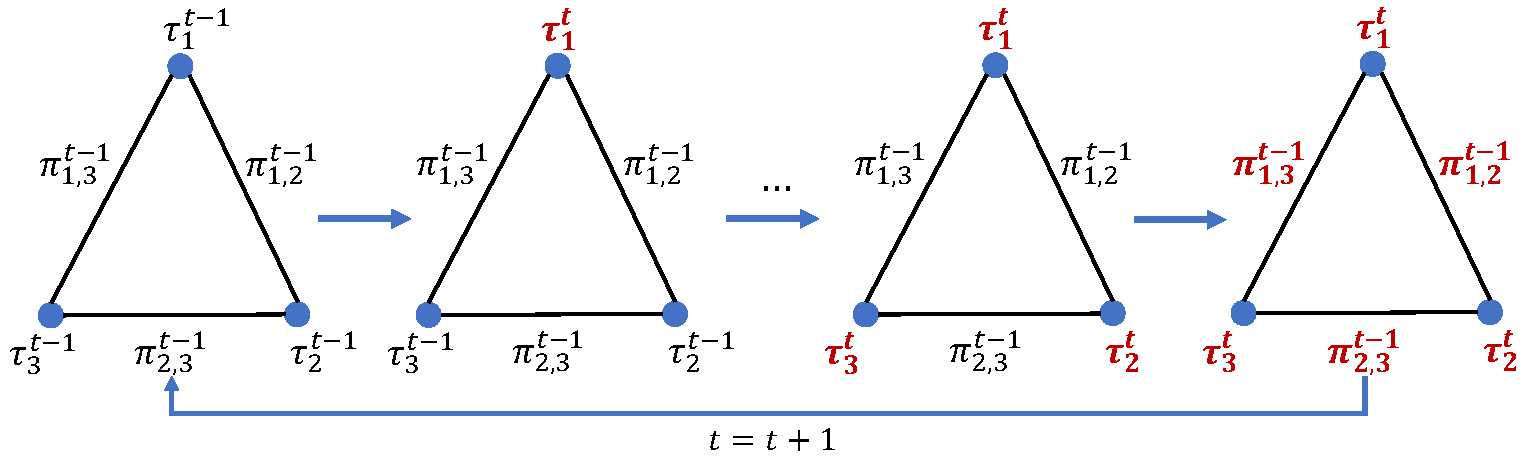
\includegraphics[width=.9\textwidth]{figs/evidence_gibbs.pdf}
   \caption{基于分块Gibbs的近似采样算法示例}
   \label{fig:evidence_gibbs}
\end{figure}

上述分块Gibbs算法采用系统遍历方法(Systematic Scan),每一步迭代常量的顺序是固定的,还可以使用随机遍历(Random Scan)方法,对于每一步$t$迭代,采用随机的常量顺序。
此外,还可以采用交替迭代方法:每一步只更新一个常量对应的随机变量组和$\mathbf{X}_B$。
由于$\mathbf{X}_B$的更新是域可提升的,且$\mathbf{X}_B$包含绝大部分随机变量(个数为$O(n^2)$,相比于剩下的$O(n)$个变量),交替更新方法可以进一步提高Gibbs采样的收敛速度。


% 3.2 可行性分析
\subsection{3.2 可行性分析}

\subsubsubsection{(1)理论基础}

\subsubsubsection{(2)完备的实验条件}

\subsubsubsection{(3)国际国内学术交流与合作}

\subsubsubsection{(4)已取得的初步进展}

\vspace{0.5 \baselineskip}
{\sihao \color{MsBlue} \kaishu 4.{\bfseries 本项目的特色与创新之处;}}
\vspace{0.5 \baselineskip}


{\sihao \color{MsBlue} \kaishu 5.{\bfseries 年度研究计划及预期研究结果}(包括拟组织的重要学术交流活动、国际合作与交流计划等)。}

% 5.1 年度研究计划
\subsubsection{{\kaishu \CJKunderline[skip=false]{5.1 年度研究计划}}}
% 5.2 预期研究成果
\subsubsection{{\kaishu \CJKunderline[skip=false]{5.2 预期研究成果}}}
% 5.3 拟组织的学术交流活动及国际合作交流计划
\subsubsection{{\kaishu \CJKunderline[skip=false]{5.3 拟组织的学术交流活动及国际合作交流计划}}}

{\color{MsBlue} \subsection{\sihao \kaishu \quad \ (二)研究基础与工作条件 }}

{\sihao \color{MsBlue} \kaishu 1.{\bfseries 研究基础}(与本项目相关的研究工作积累和已取得的研究工作成绩);}

% 1. 研究基础

\vspace{0.5 \baselineskip}
{\sihao \color{MsBlue} \kaishu 2.{\bfseries 工作条件}(包括已具备的实验条件,尚缺少的实验条件和拟解决的途径,包括利用国家实验室、国家重点实验室和部门重点实验室等研究基地的计划与落实情况);}
\vspace{0.5 \baselineskip}

% 2. 工作条件

{\sihao \color{MsBlue} \kaishu 3.{\bfseries 正在承担的与本项目相关的科研项目情况}(申请人和主要参与者正在承担的与本项目相关的科研项目情况,包括国家自然科学基金的项目和国家其他科技计划项目,要注明项目的资助机构、项目类别、批准号、项目名称、获资助金额、起止年月、与本项目的关系及负责的内容等);}

% 3. 正在承担的与本项目相关的科研项目情况

{\sihao \color{MsBlue} \kaishu 4.{\bfseries 完成国家自然科学基金项目情况}(对申请人负责的前一个已资助期满的科学基金项目(项目名称及批准号)完成情况、后续研究进展及与本申请项目的关系加以详细说明。另附该项目的研究工作总结摘要(限500字)和相关成果详细目录)。}

\vspace{0.25 \baselineskip}
{\kaishu 无。}
% \vspace{0.25 \baselineskip}

{\color{MsBlue} \subsection{\sihao \kaishu \quad \ (三)其他需要说明的情况 }}

{\sihao \color{MsBlue} \kaishu 1. 申请人同年申请不同类型的国家自然科学基金项目情况(列明同年申请的其他项目的项目类型、项目名称信息,并说明与本项目之间的区别与联系)。 }

\vspace{0.25 \baselineskip}
{\kaishu 无。}
\vspace{0.25 \baselineskip}

{\sihao \color{MsBlue} \kaishu 2. 具有高级专业技术职务(职称)的申请人是否存在同年申请或者参与申请国家自然科学基金项目的单位不一致的情况;如存在上述情况,列明所涉及人员的姓名,申请或参与申请的其他项目的项目类型、项目名称、单位名称、上述人员在该项目中是申请人还是参与者,并说明单位不一致原因。}

\vspace{0.25 \baselineskip}
{\kaishu 无。}
\vspace{0.25 \baselineskip}

{\sihao \color{MsBlue} \kaishu 3. 具有高级专业技术职务(职称)的申请人是否存在与正在承担的国家自然科学基金项目的单位不一致的情况;如存在上述情况,列明所涉及人员的姓名,正在承担项目的批准号、项目类型、项目名称、单位名称、起止年月,并说明单位不一致原因。}

\vspace{0.25 \baselineskip}
{\kaishu 无。}
\vspace{0.25 \baselineskip}

{\sihao \color{MsBlue} \kaishu 4. 其他。}

\vspace{0.25 \baselineskip}
{\kaishu 无。}
\vspace{0.25 \baselineskip}

\end{document}


